\documentclass[final,3p,times,pdflatex]{elsarticle}
\usepackage{axodraw}
\usepackage{amsmath}
\usepackage{amssymb}
\usepackage{graphicx}
\usepackage{color} 



% beginning of macros
\def\SOFTSUSY{{\tt SOFTSUSY}}
\def\code#1{\small{\tt #1}\normalsize}

\journal{Computer Physics Communications}

\begin{document}

\begin{frontmatter}

\begin{flushright}
DAMTP-2014-??
\end{flushright}

\title{Incorporating Two Loop Threshold Effects and Three Loop Gauge and
  Yukawa Renormalisation Group Equations in the Calculation of the Spectrum
  of the Minimal Supersymmetric Standard Model: {\tt SOFTSUSY3.5.0}}

\author[damtp]{B.C.~Allanach}
\author[valencia]{R.R.~de Austri\corref{cor1}}
\ead{rruiz@ific.uv.es}
\cortext[cor1]{Corresponding author}
\author[dunba]{A.~Bednyakov}

\address[damtp]{DAMTP, CMS, University of Cambridge, Wilberforce road,
  Cambridge, CB3  0WA, United Kingdom}
\address[valencia]{Instituto de Física Corpuscular | Parque Científico,
  C/Catedrático José Beltrán, 2 | E-46980 Paterna, Spain} 
\address[dubna]{Joint Institute for Nuclear Research, 141980, Dubna, Russia}

\begin{abstract}
  Previous minimal supersymmetric standard model public spectrum calculators
  contain two-loop 
  renormalisation group equations and one-loop threshold corrections to the
  gauge and Yukawa couplings. Here, we explore the effects of three-loop
  renormalisation group equation terms, leading two-loop threshold
  corrections are incorporated to the third family Yukawa couplings and the
  strong coupling constant.
  We illustrate our results in the constrained minimal supersymmetric standard
  model (CMSSM). 
  At a generic CMSSM point, some of the sparticle masses change by around
  3$\%$ and the 
  lightest CP-even Higgs mass by around 2-3 GeV. 
  The changes can be much greater in the fixed point region of the CMSSM at
  high values of $m_0$, a region which has become more attractive, given the
  emprirical Higgs mass constraints. 
  We also provide detail on the
  approximations used. The additional higher order corrections have been
  incorporated into {\tt SOFTSUSY3.5.0}, and we provide details on how to
  compile and use the program. 
\end{abstract}

\begin{keyword}
sparticle, 
MSSM
\PACS 12.60.Jv
\PACS 14.80.Ly
\end{keyword}
\end{frontmatter}

\section{Program Summary}
\noindent{\em Program title:} \SOFTSUSY{}\\
{\em Program obtainable   from:} {\tt http://softsusy.hepforge.org/}\\
{\em Distribution format:}\/ tar.gz\\
{\em Programming language:} {\tt C++}, {\tt fortran}\\
{\em Computer:}\/ Personal computer.\\
{\em Operating system:}\/ Tested on Linux 3.x\\
{\em Word size:}\/ 64 bits.\\
{\em External routines:}\/ At least {\tt GiNaC1.3.5} and {\tt CLN1.3.1}\\
{\em Typical running time:}\/ A minute per parameter point.\\
{\em Nature of problem:}\/ Calculating supersymmetric particle spectrum and
mixing parameters in the next-to-minimal minimal supersymmetric standard
model. The solution to the renormalisation group equations must be consistent
with boundary conditions on supersymmetry breaking parameters, as
well as on the weak-scale boundary condition on gauge 
couplings, Yukawa couplings and the Higgs potential parameters.\\
{\em Solution method:}\/ Nested iterative algorithm. \\
{\em Restrictions:} \SOFTSUSY~will provide a solution only in the
perturbative regime and it
assumes that all couplings of the model are real
(i.e.\ $CP-$conserving). If the parameter point under investigation is
non-physical for some reason (for example because the electroweak potential
does not have an acceptable minimum), \SOFTSUSY{} returns an error message.\\
{\em CPC Classification:} 11.1 and 11.6.\\
{\em Does the new version supersede the previous version?:} Yes.\\
{\em Reasons for the new version:} Major extension to include additional two
and three-loop terms.\\
{\em Summary of revisions:} 
All quantities in the minimal supersymmetric standard model are extended to
have three-loop renormalisation group equations in the limit of real
parameters and leading two-loop threshold
corrections are incorporated to the third family Yukawa couplings and the
strong gauge coupling. 
\newpage

\section{Introduction}

The recent discovery of the Higgs boson~\cite{Aad:2012tfa,Chatyrchan:2012ufa}
and the measurement of its mass at around 
125-126 GeV~\cite{ATLAS-CONF-2013-014} solidify the important and well-known
question of how its mass is 
stabilised with respect to quantum corrections, which are expected to be of
order the largest fundamental mass scale divided by the 16$\pi^2$ loop factor.
In particular, the Planck mass at $\sim 10^{19}$ GeV from gravitational
corrections is expected to be the largest such relevant mass scale. 
However, since a quantum field theoretic description of gravity does not
exist it is possible, if not expected, that our effective field theory
description breaks down and such huge corrections are absent
for some reason. 
In any case, mass scales associated with the string scale $\sim 10^{17}$ GeV
or the GUT scale $\sim 10^{16}$ GeV reintroduce the question of stability of
the Higgs mass.  
Imposing softly-broken supersymmetry upon the Standard Model provides a
well-known answer to this question, and this approach has been pursued
with vigour in the literature and at various high energy colliders (see, for
example, Refs.~\cite{Aad:2013wta,Chatrchyan:2014lfa}), where 
the Standard Model particles' supersymmetric partners predicted are being
searched for. To date, no unambiguous direct collider signals of
supersymmetric particles have been found, and a significant portion of the
most interesting parameter space has been ruled out. 
In order to rule a parameter point out, one predicts sparticle masses using
a supersymmetric spectrum generator and then simulates various collisions,
comparing to data to see if the predicted signals are significantly excluded
or not (or conversely, to see if there is evidence statistically significant
enough to claim a signal).

There are currently several available sparticle generators: {\tt
  ISAJET}~\cite{Paige:2003mg}, {\tt 
  SOFTSUSY}~\cite{Allanach:2001kg,Allanach:2009bv,Allanach:2011de,Allanach:2013kza}, 
{\tt SPheno}~\cite{Porod:2003um},
{\tt SUSEFLAV}~\cite{Chowdhury:2011zr} and
{\tt SUSPECT}~\cite{Djouadi:2002ze}. Even specialising to the minimal
supersymmetric standard model (MSSM) with real parameters, 
they have slightly different
approximations, resulting in numerical predictions that are not
identical~\cite{Allanach:2003jw,Allanach:2004rh,Belanger:2005jk}. 
Even when calculations have at the same headline order of approximation (for
example, `two-loop RGEs and one-loop threshold corrections at $M_Z$),
legitimate differences can result from the fact that higher order corrections
contribute to the calculation implicitly in different ways. 
If we take the example of a one-loop threshold correction to, for example, 
the prediction of the stop mass, there are various contributions from Standard
Model and supersymmetric particles. If we consider an internal loop with
say a gluino propagator, which mass do we use for the gluino? One achieves
numerically distinct results if one uses two of the obvious choices: the
pole mass or the modified dimensional reduction ($\overline{DR}$) running
mass. The difference between the two prescriptions is a two-loop threshold
effect, and so either choice is allowed if one is working only at one loop.
Such choices occur hundreds of times within the calculation, multiplying the
poissibilities for numerical differences. Thus, the numerical differences
between the spectrum calculators gives a rough estimate of the size of
theoretical uncertainties associated with the calculation. 

The constrained minimal supersymmetric standard model makes a simplying
assumption about the supersymmetry breaking terms: each soft SUSY breaking
scalar mass is set to a common value $m_0$ at a high scale $M_{GUT}$, the
gaugino masses are set to a common value $M_{1/2}$ at $M_{GUT}$ and the 
SUSY breaking trilinear scalar couplings are all fixed to a value $A_0$ at
$M_{GUT}$. The other relevant parameters are $\tan \beta$, the ratio of the
two Higgs vacuum expectation values, and the sign of a parameter $\mu$ that
appears in the Higgs potential (its magnitude is fixed minimisation of the
Higgs potential in order to predict the empirically measured central value of
the $Z^0$ boson mass).

The obvious way to reduce such a theoretical uncertainty is to incorporate the
higher order effects, pushing the associated theoretical uncertainty to even
higher orders.
That is what we have done for the present paper: we have
picked some available higher order terms that are expected to affect the
predictions of the spectrum mass calculation, and included them in
{\tt SOFTSUSY3.5.0}. The previous version of the program, {\tt SOFTSUSY3.4.1}, 
contained two-loop RGEs and one-loop threshold corrections. 
The higher order terms that we have included to the MSSM spectrum
calculation are: 
\begin{enumerate}
\item
Three-loop RGEs to all soft and supersymmetry preserving parameters, 
assuming that they are real. The supersymmetric parameters contain the
possibility of full three-family mixing. The three-loop contribution to the 
soft-breaking MSSM parameters are calculated in the dominant third family
approximation. 
\item
The following two-loop threshold corrections:
\begin{enumerate}
\item
$\mathcal O(\alpha_s^2)$ corrections to $m_t$, which we call $\Delta m_t$
\item
$\mathcal O(\alpha_s^2)$, $\mathcal O(\alpha_s Y_b^2)$, $\mathcal O(\alpha_s
Y_t^2)$ corrections to $\alpha_s$. Collectively, we call these corrections
$\Delta \alpha_s$.
\item
$\mathcal O(\alpha_s^2)$, $\mathcal O(\alpha_s Y_b^2)$, $\mathcal O(\alpha_s
Y_b^2)$ corrections to $m_b$. Also included are $\mathcal O(Y_\tau^4)$
corrections to $m_\tau$. 
{\bf Sascha is this correct?} We call this
collection of corrections $\Delta m_b, m_\tau$.
\end{enumerate}
\end{enumerate}
None of these terms have been, to our knowledge, included in any publicly
available programs before. 

The effect of the three-loop RGEs upon the Snowmass Benchmark
Points~\cite{Allanach:2002nj} were presented and studied in
Ref.~\cite{Jack:2004ch} 
without the inclusion of the two-loop threshold effects. 
The three-loop RGEs are enhanced by a large logarithm $\log M_{GUT}/M_Z$,
which effectively promotes them to the size of a two-loop threshold effect. 
Thus the additional higher order terms that were included in
Ref.~\cite{Jack:2004ch} were of the same order of other terms that were
missing in the calculation. Effects upon sparticle mass predictions of around
1-2$\%$ were typically found, although one point studied did have an 8$\%$
difference in the light stop mass at the SPS5 point. 
However, 
{\bf TALK ABOUT JJ AND SASCHA'S RESULTS AND ANY DIFFERENCE WE HAVE}.


\section{Increases in Calculational Accuracy}
SCALE DEPENDENCE?

\section{Effect on Sparticle Spectra}
\subsection{Dissection of the higher order effects at benchmark points}
% omega_{CDM h^2}=1.220000e-01
\begin{table}
\begin{center}
\begin{tabular}{|c|c|ccccccc|}\hline
Threshold & RGEs  & $m_h$  & $m_{\tilde g}$ & $m_{{\tilde q}}$ & $m_{\chi_1^0}$  & $m_{\chi_2^0}$ & $m_{\chi_3^0}$ & $m_{\chi_4}^0$ \\ \hline
None               & 2 & 125.0 & 2015 & 7322 &  364 &  705 & 1298 &1303\\
$\Delta \alpha_s$  & 2 &  +0.6 & -49.4 &  -2.2 &  +1.7 &  +5.2 & +565.0 &+562.4\\
$\Delta m_t$      & 2 & N/A & N/A & N/A & N/A & N/A & N/A & N/A  \\
$\Delta m_b, m_\tau$& 2 &  +0.1 &  -0.6 &  -0.5 &  -0.1 &  -0.1 & +24.3 &+24.1\\
$\Delta$ All      & 3 &  -2.6 & -49.5 &  -6.6 & -18.8 & -294.1 & -883.1 &-583.9\\

%
\hline&& $m_{{\tilde t}_L}$  & $m_{{\tilde t}_R}$ &$m_{{\tilde b}_L}$&$m_{{\tilde b}_R}$&$m_{{\tilde \tau}_L}$&$m_{{\tilde \tau}_R}$&$m_{\chi_1}^\pm$ \\ \hline
None             & 2 &4948 & 4216 & 4943 & 5559 & 6265 & 5095 & 705\\
$\Delta \alpha_s$  & 2 & -68.3 & -138.6 & -68.2 & -17.7 &  +0.7 &  +1.6 & +5.2\\
$\Delta m_t$      & 2 & N/A & N/A & N/A & N/A & N/A & N/A & N/A \\
$\Delta m_b, m_\tau$& 2 & +58.1 &  -4.8 & +58.4 & +108.4 &  +3.8 & +10.2 & -0.1\\
$\Delta$ All      & 3 &  +6.7 & +94.6 &  +6.8 & -63.7 &  +6.7 & +15.8 &-305.6\\

%
\hline      &  & $g_3(M_{SUSY})$ & $Y_t(M_{SUSY})$ &  $Y_b(M_{SUSY})$ & $Y_\tau(M_{SUSY})$  & $\mu(M_{SUSY})$    & $\Omega_{CDM} h^2$ & $\sigma_{SUSY}^{TOT}$\\ \hline
 None                   & 2 & 1.001 & 0.815 & 0.636 & 0.512 & 1278 &  91.0 &   1.2\\
$\Delta \alpha_s$  & 2 & -0.020 & +0.011 & -0.002 & +0.000 & +564 & +255.0 &  +0.4\\
$\Delta m_t$      & 2 & N/A & N/A & N/A & N/A & N/A & N/A& N/A\\
$\Delta m_b, m_\tau$& 2 & -0.000 & -0.000 & -0.020 & -0.001 &  +24 & +11.000 &  +0.0\\
$\Delta$ All      & 3 & -0.020 & -0.020 & +0.004 & -0.001 & -881 & -90.9 & +0.4\\

%
\hline&& $M_{GUT}/10^{16}$& $1/\alpha_{GUT}$&$\Delta (\alpha)$ & $\Delta Y_{b\tau}$ & $\Delta Y_{tb}$&& \\ \hline None                   & 2 & 1.669 & 25.704 & -0.000 & -0.132 & 0.167& & \\
$\Delta \alpha_s$  & 2 &  -0.037 &  0.046 &  -0.001 & -0.123 &0.197 & & \\
$\Delta m_t$  & 2 & N/A & N/A & N/A & N/A &N/A  & &\\
$\Delta m_b,m_\tau$  & 2 &  0.001 &  -0.001 &  -0.000 & -0.143 &0.184 & & \\
$\Delta$ All  & 3 &  0.097 &  -0.078 &  -0.001 & -0.120 &0.140 & & \\
\hline
\end{tabular}
\end{center}

\caption{\label{tab:cmssm} Differences due to the highest order terms
  (three-loop 
  RGEs for gauge and Yukawa couplings and two-loop threshold corrections to
  third family fermion masses and $g_3$) on various predicted quantities 
  in the focus point of the CMSSM for $m_0=7130$ GeV, $M_{1/2}=800$ GeV,
  $A_0=-6000$ GeV, $\tan \beta=50$, $\mu>0$.
  We display massive quantities in units of GeV.
  The first column details which higher order threshold corrections are
  included: `None'   meaning that only those present in {\tt
    SOFTSUSY3.4.1}~are included, `$\Delta \alpha_s$' meaning that the 2-loop
  threshold corrections to $\alpha_s$ are also included. `$\Delta m_t$' means
  that only the 2-loop threshold corrections to $m_t$ are included, whereas
  $\Delta m_b, 
  m_\tau$ means that only the two-loop threshold corrections to $m_t$ and
  $m_b$ are included. `All' means that all available two-loop threshold
  corrections to $\alpha_s$, $m_t$ and $m_b$ are included.
  `N/A' means that electroweak
  symmetry was not broken, and so reliable results cannot be reported. 
  $m_{\tilde q}$ refers to the average mass of the squarks of the first two
  families. 
  The rows marked with a $\Delta$ show the {\em change} in
  the mass from the {\tt SOFTSUSY3.4.1} result. The column labeled `RGEs'
  shows the number of loops used in the MSSM RGEs. }
\end{table}
In Table~\ref{tab:cmssm}, we show the effects of the higher order terms for a
CMSSM parameter point that is in the high $\tan \beta$ focus point region:
($m_0=7130$ GeV, $M_{1/2}=800$ GeV, $A_0=-6000$ GeV,
$\tan \beta=50$, sign $\mu>0$) with 
rather attractive properties: it has a high lightest CP even Higgs mass of
122.3 GeV, within $1\sigma$ of the experimental
central value, once theoretical uncertainties (estimated to be around $\pm3$
GeV~\cite{Allanach:2004rh}) 
have been taken into account.
It also has attractive dark matter properties: $\Omega_{CDM} h^2=0.099$ is
close to the central value inferred from cosmological observations. Aside from
that, the gluino and squark masses are heavy enough so as to not be ruled out
by the LHC7/8 TeV data. Apart from these phenomenologically advantageous
properties, the point has a high value of $\tan \beta=50$, which may give the 
bottom and tau Yukawa corrections a higher impact than if $\tan \beta$ were
smaller (at higher values of $\tan \beta$, the bottom and tau Yukawa couplings
are roughly proportional to $\tan \beta$).
We split the various higher order corrections up in
the table: the `base' calculation is always considered to be {\tt
  SOFTSUSY3.4.1}, which does not contain the higher order corrections. 
We see that the row $\Delta m_t$, that includes 2-loop threshold corrections
to $m_t$ coming from strong SUSY QCD corrections only contains `N/A' entries,
indicating that the calculation failed in this approximation because
electroweak symmetry was not broken successfully. {\bf EWSB equation}.
At the focus point,
the predicted value of $\mu$ derived from electroweak symmetry breaking is
known to 
depend extremely sensitively upon the precise value of the top Yukawa
coupling. 
The parameter point appears to agree with the experimental result on the Higgs
mass (which, in the CMSSM at high masses, acts to a good approximation with
identical couplings to the Standard Model Higgs)
to within the one 1$\sigma$ level according to the {\tt SOFTSUSY3.4.1}
calculation. However, one would discard the point based on the predicted value
of 95 for $\Omega_{CDM} h^2$, which disagrees with the cosmologically inferred
value by hundreds of sigma. On the other hand, including all of the high order
corrections (`$\Delta$ All'), we see that the Higgs mass lowers somewhat, and
the dark matter 
relic density is predicted to be the cosmologically acceptable value of 0.99
once all of the higher order corrections are included.
The two-loop threshold corrections to the bottom and tau Yukawa couplings 
have a very small effect: smaller than 0.1 GeV for most of the sparticle
masses, despite the fact that the Yukawa couplings themselves are of order the
top Yukawa coupling. 
Two-loop threshold corrections to the strong gauge coupling have a significant
effect upon some of the sparticle masses: particularly $m_{\chi_3^0}$ and
$m_{\chi_4^0}$. {\bf neutralino mass equation}.
These two masses are controlled to leading order by $\mu$,
which in turn is affected sensitively by the top Yukawa coupling. 
The top Yukawa coupling is changed by the different value of $\alpha_s$
through renormalisation group effects. {\bf one-loop $Y_t$ RGE}.
(Higgs mass uncertainty).

\begin{table}
\begin{center}
\begin{tabular}{|c|c|ccccccc|}\hline
Threshold & RGEs  & $m_h$  & $m_{\tilde g}$ & $m_{{\tilde q}}$ & $m_{\chi_1^0}$  & $m_{\chi_2^0}$ & $m_{\chi_3^0}$ & $m_{\chi_4}^0$ \\ \hline
None               & 2 & 117.1 & 1088 & 1042 &  790 & 2431 & 2500 &2551\\
$\Delta \alpha_s$  & 2 &  +0.5 &  -3.4 &  -1.7 &  +0.0 &  -0.1 &  -0.2 & -0.1\\
$\Delta m_t$      & 2 &  -2.9 &  +0.0 &  +0.0 &  +0.0 &  +0.3 &  +0.9 & +0.6\\
$\Delta m_b, m_\tau$& 2 &  +0.0 &  +0.0 &  +0.0 &  -0.0 &  +0.0 &  +0.0 & +0.0\\
$\Delta$ All      & 3 &  -2.1 &  -3.3 &  -1.6 &  +0.0 &  +0.2 &  +0.6 & +0.4\\

%
\hline&& $m_{{\tilde t}_L}$  & $m_{{\tilde t}_R}$ &$m_{{\tilde b}_L}$&$m_{{\tilde b}_R}$&$m_{{\tilde \tau}_L}$&$m_{{\tilde \tau}_R}$&$m_{\chi_1}^\pm$ \\ \hline
None             & 2 &2557 & 2528 & 2554 & 2526 & 2523 & 2500 &2431\\
$\Delta \alpha_s$  & 2 &  -0.8 &  -0.8 &  -0.8 &  -0.9 &  -0.0 &  +0.0 & -0.1\\
$\Delta m_t$      & 2 &  -0.4 &  +0.1 &  +0.1 &  -0.0 &  +0.0 &  -0.0 & +0.3\\
$\Delta m_b, m_\tau$& 2 &  +0.0 &  +0.0 &  -0.2 &  +0.3 &  +0.0 &  -0.0 & +0.0\\
$\Delta$ All      & 3 &  -1.1 &  -0.7 &  -0.9 &  -0.6 &  +0.0 &  -0.0 & +0.2\\

%
\hline      &  & $g_3(M_{SUSY})$ & $Y_t(M_{SUSY})$ &  $Y_b(M_{SUSY})$ & $Y_\tau(M_{SUSY})$  & $\mu(M_{SUSY})$    & $\Omega_{CDM} h^2$ & $\sigma_{SUSY}^{TOT}$\\ \hline
 None                   & 2 & 1.040 & 0.834 & 0.124 & 0.100 & 2500 &  10.9 & 1682.2\\
$\Delta \alpha_s$  & 2 & -0.014 & +0.006 & +0.001 & -0.000 &   +0 &  -0.1 & +32.1\\
$\Delta m_t$      & 2 & +0.000 & -0.025 & +0.000 & +0.000 &   +0 &  +0.0 &  +0.0\\
$\Delta m_b, m_\tau$& 2 & +0.000 & +0.000 & -0.004 & +0.000 &   +0 & +0.000 &  +0.0\\
$\Delta$ All      & 3 & -0.013 & -0.016 & -0.002 & +0.000 &   +0 &  -0.1 &+32.1\\
\hline
\end{tabular}
\end{center}

\caption{\label{tab:pmssm}  Differences due to the highest order terms
  (three-loop 
  RGEs for gauge and Yukawa couplings and two-loop threshold corrections to
  third family fermion masses and $g_3$) on various predicted quantities 
  in the phenomenological MSSM point 1.6~\cite{AbdusSalam:2011fc}. The first
  column details which higher order threshold corrections are 
  included: `None'   meaning that only those present in {\tt
    SOFTSUSY3.4.1}~are included, `$\Delta \alpha_s$' meaning that the 2-loop
  threshold corrections to $\alpha_s$ are also included. `$\Delta m_t$' means
  that only the 2-loop threshold corrections to $m_t$ are included, whereas
  $\Delta m_b, 
  m_\tau$ means that only the two-loop threshold corrections to $m_t$ and
  $m_b$ are included. `All' means that all available two-loop threshold
  corrections to $\alpha_s$, $m_t$ and $m_b$ are included.
  `N/A' means that electroweak
  symmetry was not broken, and so reliable results cannot be reported. 
  $m_{\tilde q}$ refers to the average mass of the squarks of the first two
  families. 
  The rows marked with a $\Delta$ show the {\em change} in
  the mass from the {\tt SOFTSUSY3.4.1} result. The column labeled `RGEs'
  shows the number of loops used in the MSSM RGEs. }
\end{table}
We now wish to decouple the three-loop RGE effects from the two-loop threshold
effects as far as possible while still giving a valid prediction for a point
in MSSM parameter space. This can be achieved by studying the spectrum from a
point in phenomenological MSSM (pMSSM) parameter space, where supersymmetry
breaking 
boundary conditions are imposed already at the SUSY breaking scale, defined to 
be $\sqrt{m_{{\tilde t}_1} m_{{\tilde t}_2}}$. We use the point pMSSM1.6 from
Ref.~\cite{AbdusSalam:2011fc}, which is defined to have all scalar trilinear
couplings 0, the first two generation squark mass, 
the tree-level bino and gluino masses all set to 800 GeV and a tree-level gluino
mass of 960 GeV. The tree-level wino mass, $\mu$ and the pseudoscalar Higgs
pole mass and all other tree-level squark and slepton masses are fixed to 2500
GeV. The aim of using the pMSSM is to reduce the effects of the RGEs in order
to study the threshold contributions more cleanly. However, we cannot
eliminate RGE effects completely because there is still running between 
$M_Z$ and $M_{SUSY} \sim 2.5$ TeV, however they are small, being of order
$1/(16 \pi^2) \log M_{SUSY}/M_Z$, i.e.\ not enhanced by large logarithms,
unlike the CMSSM case above. 
We see that the lightest CP-even Higgs mass prediction decreases by 2.1 GeV,
mainly because of the  corrections to the top mass. The high order strong
corrections to $\alpha_s$ reduce
squark and gluino masses at the per-mille level, which will only have a very
small effect on collider signatures. 
We see that the RGE corrections do induce a small additional change: but it is
at the per-mille or smaller level for this point.
The sparticle mass predictions only change by a
very small amount, which is contrary to the case of the focus-point CMSSM
(which is 
admittedly very sensitive to small changes in the top Yukawa coupling) that is
shown in Table~\ref{tab:cmssm}. However, we shall show next that even for more
generic CMSSM points, there are typically changes in the spectra of 2-3$\%$.
We conclude that in this point of the pMSSM, the higher order effects are not
needed for collider studies except for those involving the lightest CP-even
Higgs. We find it likely, where no input mass parameters are lighter
than 700 GeV that this conclusion will hold more generally for the
pMSSM because of sparticle decoupling in the corrections. 
Obviously, to be sure of this conclusion, one should check the point's
robustness with respect to the higher order effects. 

\subsection{CMSSM parameter scans}

We now perform a scan over CMSSM parameter space in order to examine the kind
of behaviour expected more generically from the higher order corrections, and
also to foretell possible effects on SUSY phenomenology. We choose the
$m_0-M_{1/2}$ plane with $\mu>0$, $\tan \beta=30$ and $A_0=-2m_0$, which was
recently used by ATLAS to place bounds upon the CMSSM from various LHC 8
TeV searches~\cite{}. 

In Fig.~\ref{fig:}, we show some contours of important MSSM particle masses as
well as their relative change due to the higher order corrections. The region
below the dashed line is excluded by either one or both of the most
restrictive ATLAS SUSY searches~\cite{ATLAS-CONF-2013-047,Aad:2013wta}. 
\begin{figure}
\unitlength=1in
\begin{center}
\begin{picture}(6,7.8)
  \put(-0.75,2.8){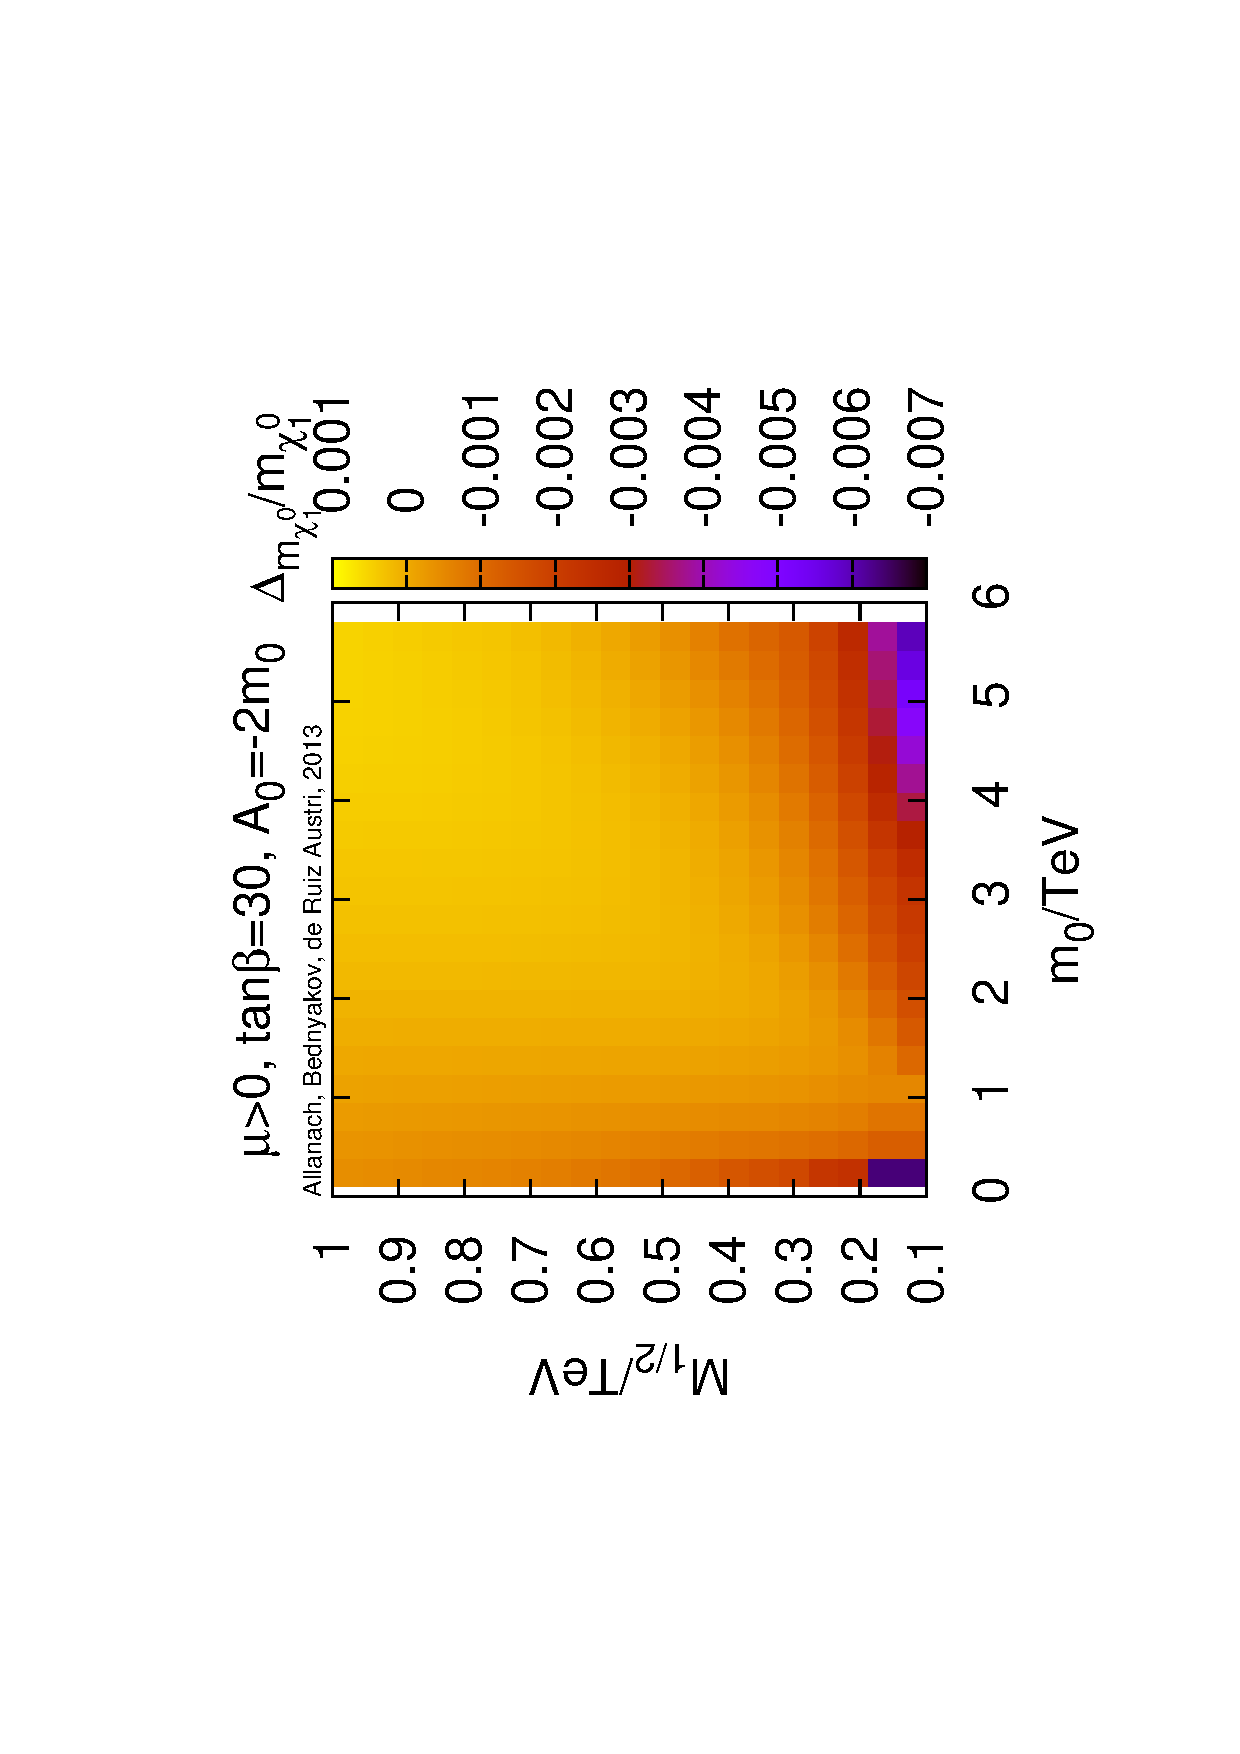
\includegraphics[angle=270,width=0.7\textwidth]{atlasScanMneut1}}
  \put(0.08,2.24){
\includegraphics[angle=270,width=0.45\textwidth]{atlasScanMneut12}}
  \put(0.08,2.24){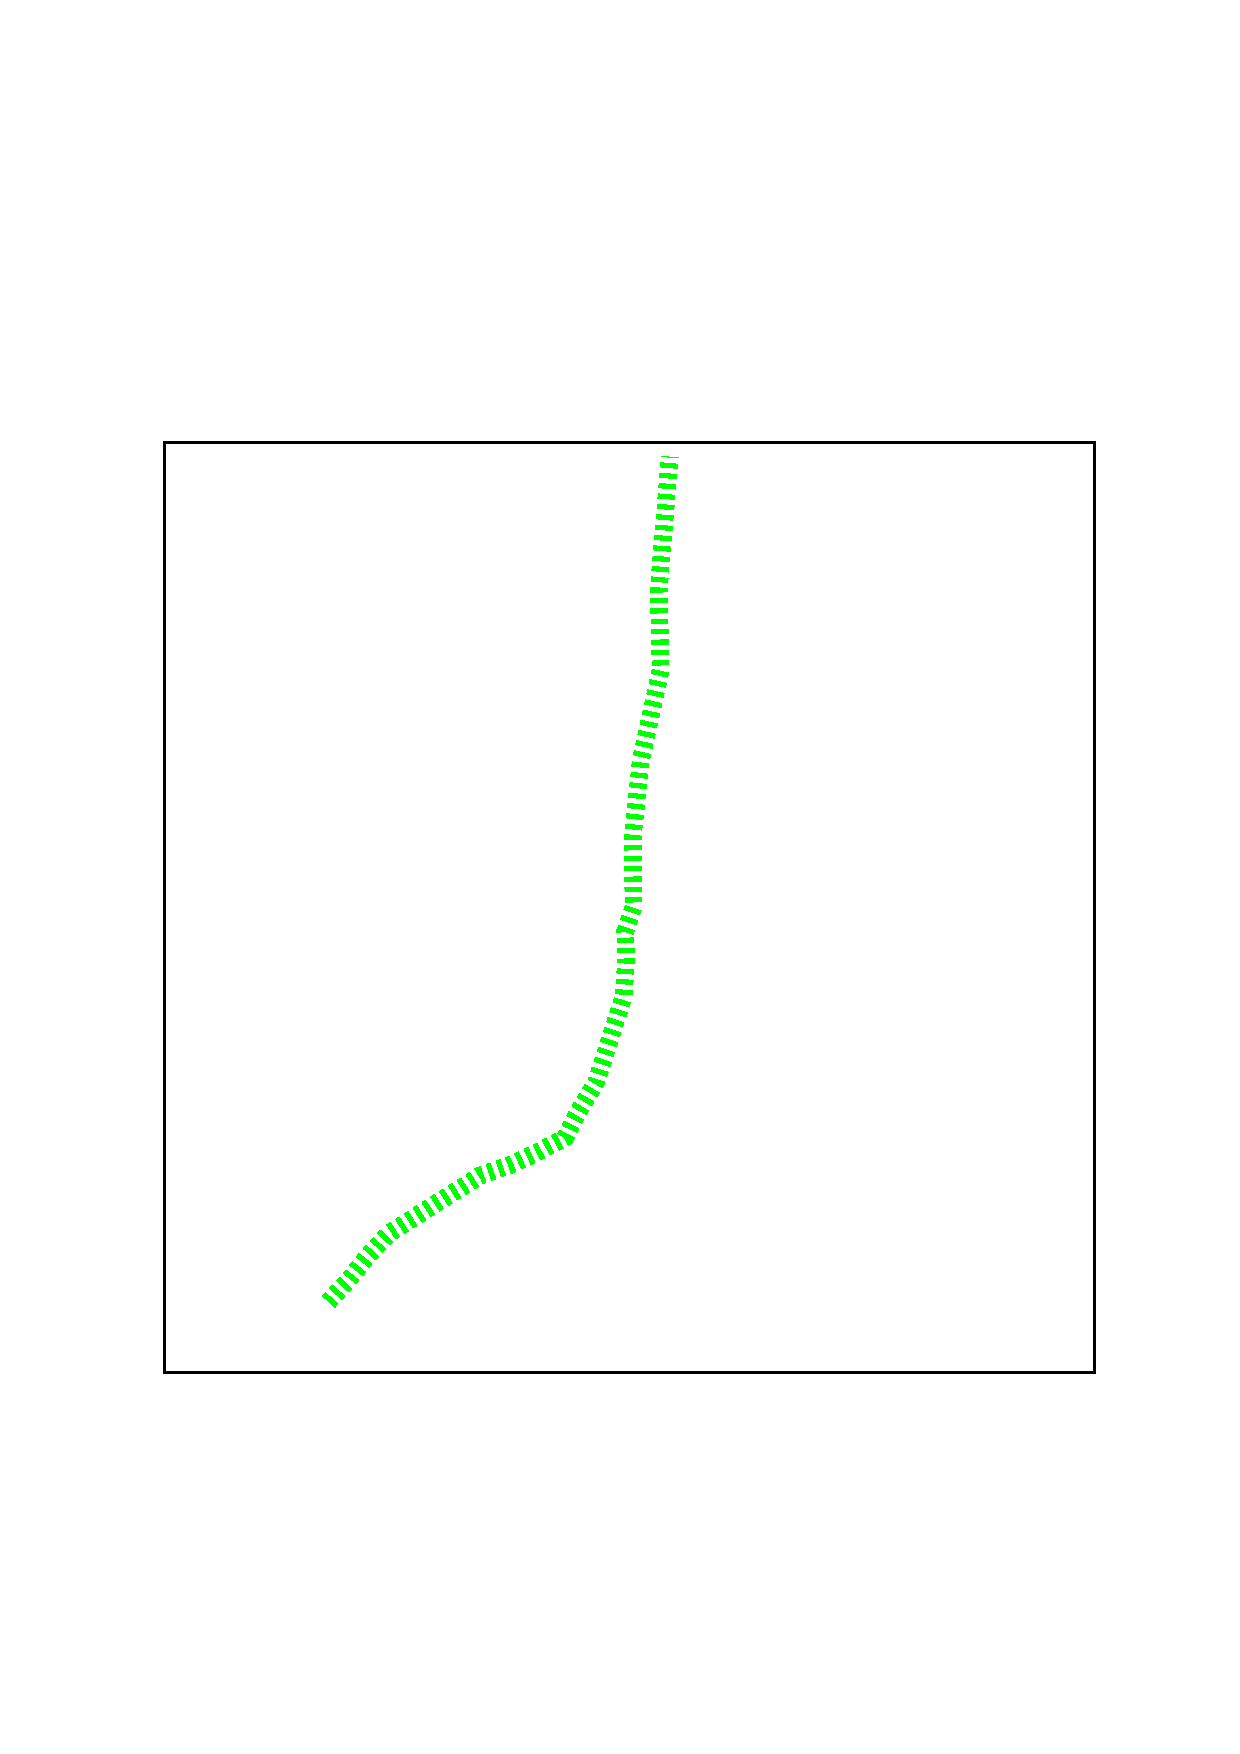
\includegraphics[angle=270,width=0.45\textwidth]{atlasExcl}}
  \put(-0.75,5.5){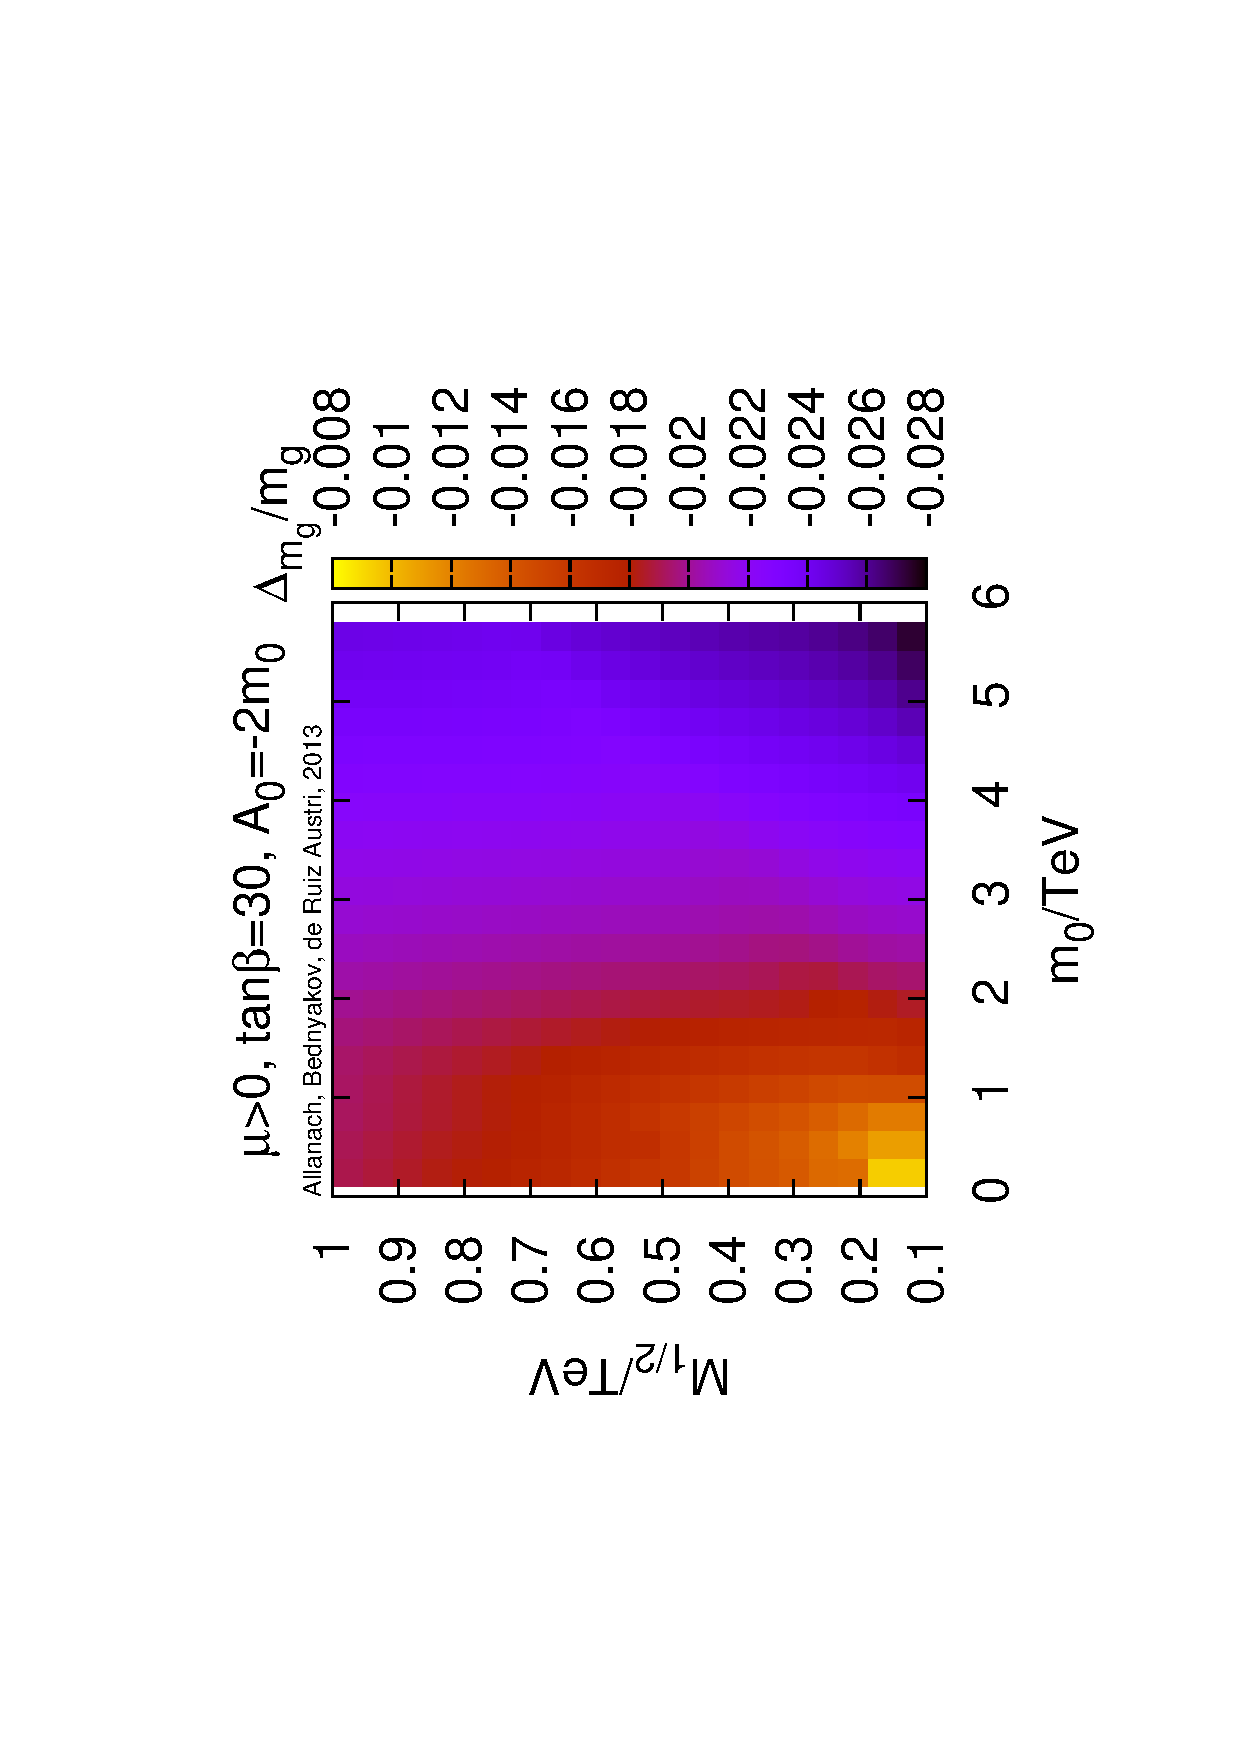
\includegraphics[angle=270,width=0.7\textwidth]{atlasScanMg}}
  \put(0.08,4.94){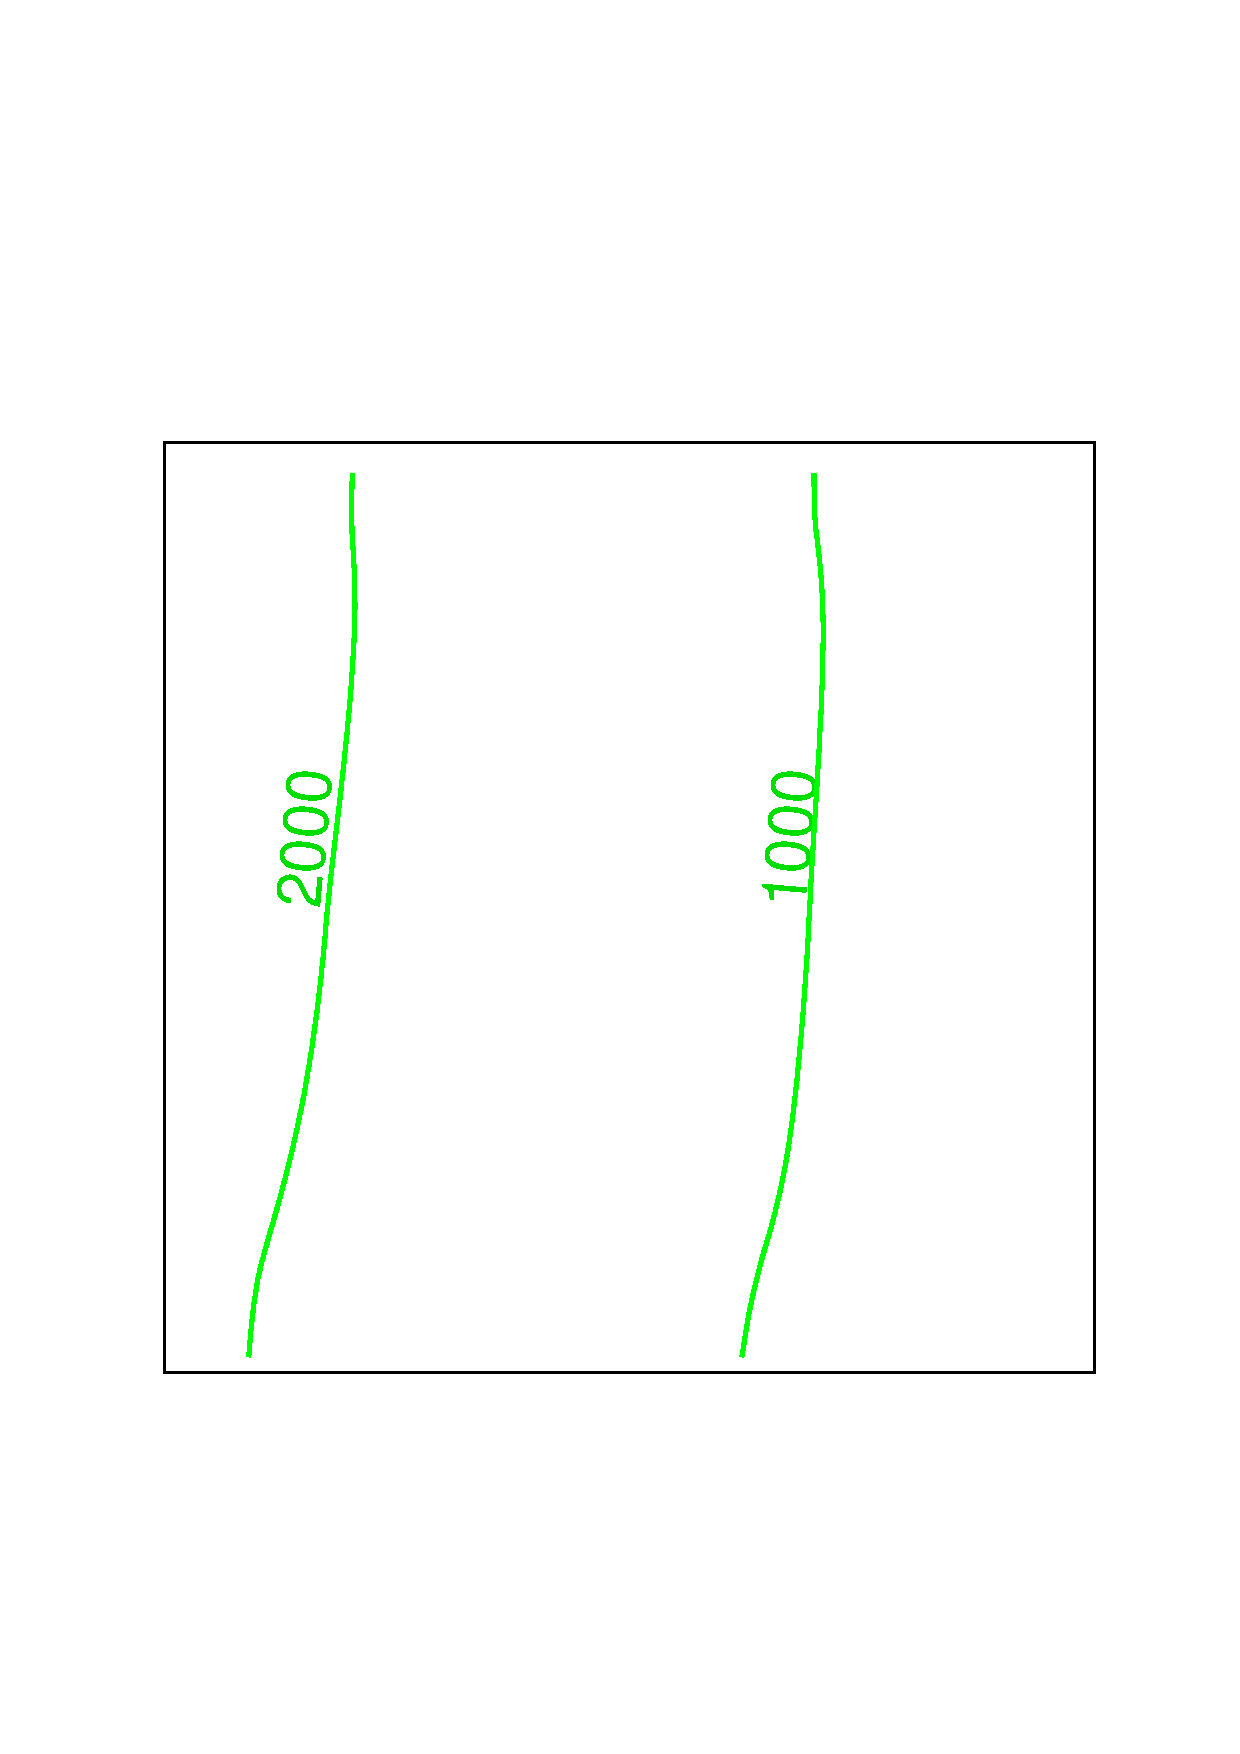
\includegraphics[angle=270,width=0.45\textwidth]{atlasScanMg2}}
  \put(0.08,4.94){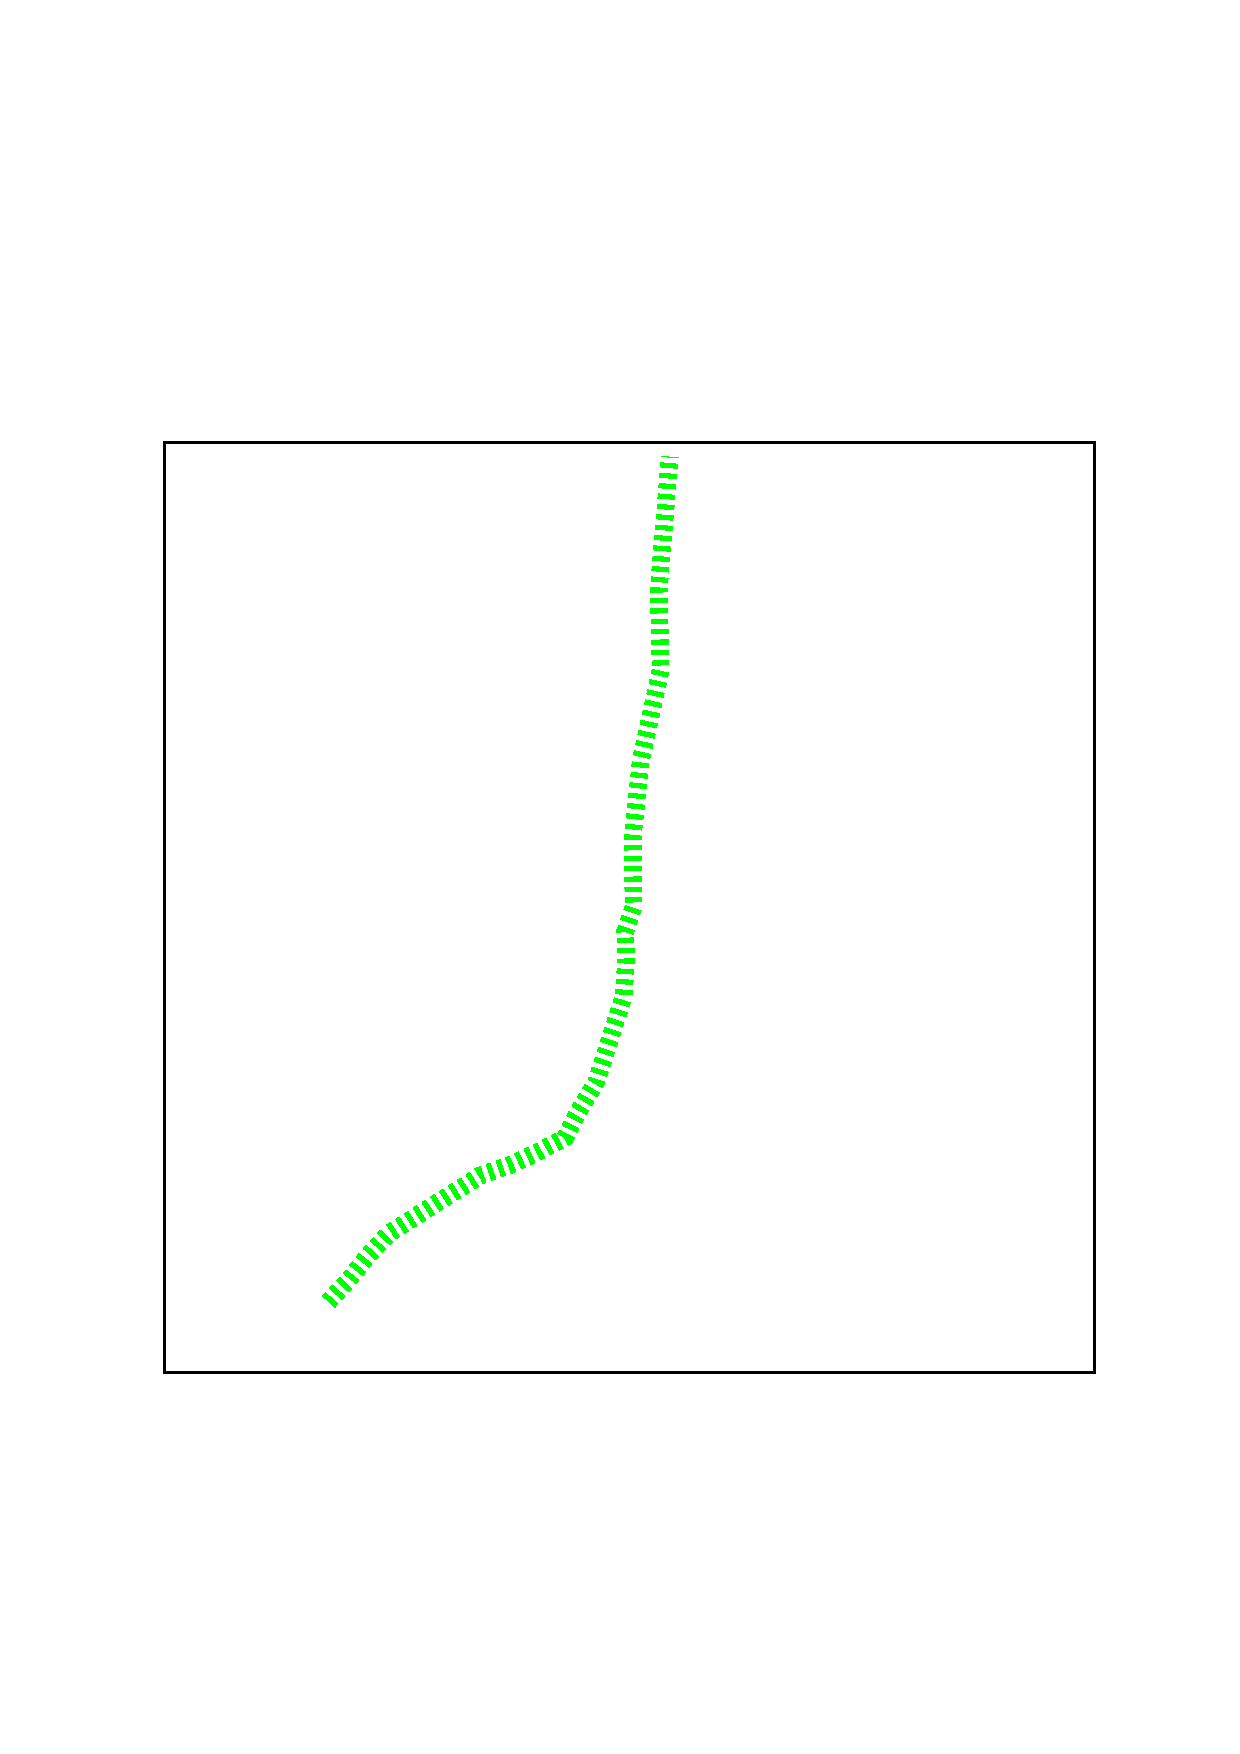
\includegraphics[angle=270,width=0.45\textwidth]{atlasExcl}}
  \put(2.4,2.8){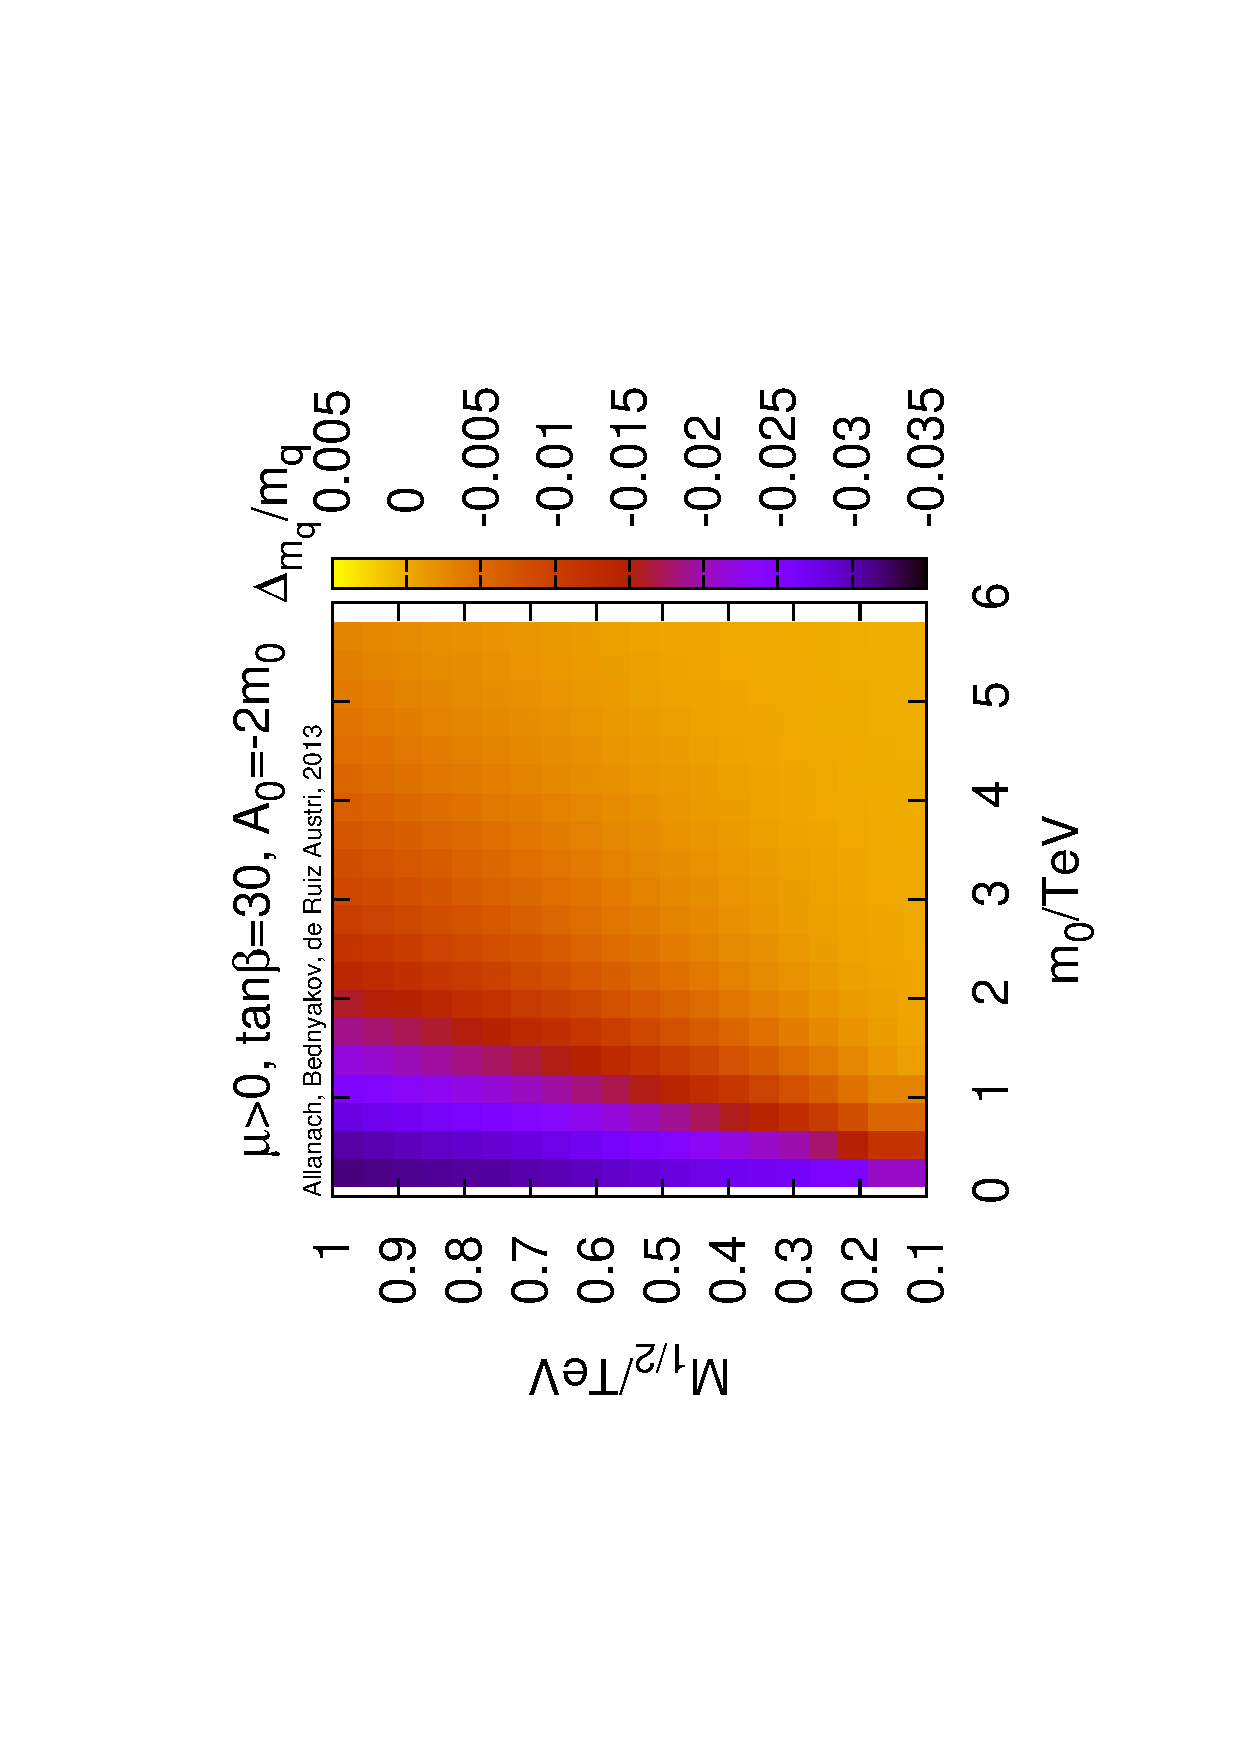
\includegraphics[angle=270,width=0.7\textwidth]{atlasScanMq}}
  \put(3.22,2.24){
\includegraphics[angle=270,width=0.45\textwidth]{atlasScanMq2}}
  \put(3.22,2.24){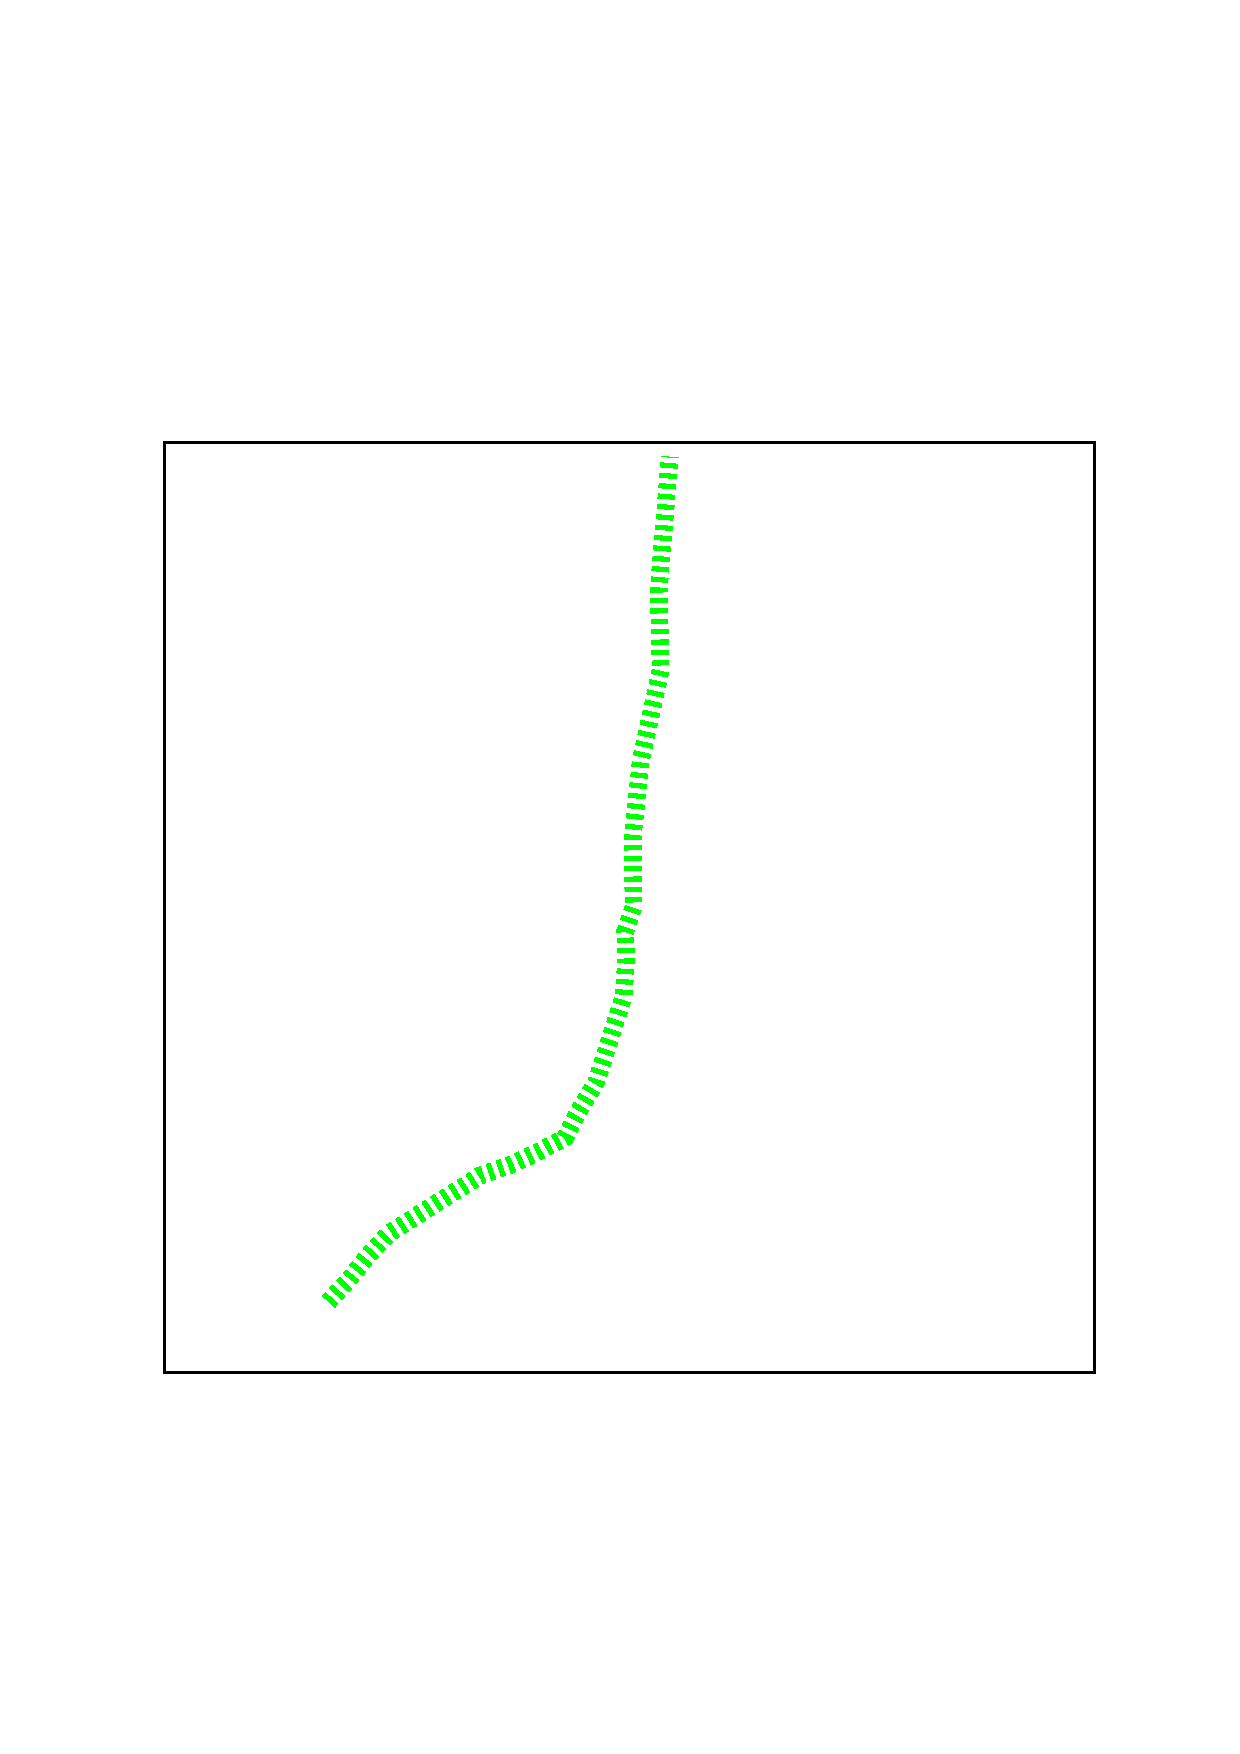
\includegraphics[angle=270,width=0.45\textwidth]{atlasExcl}} 
\put(2.4,5.5){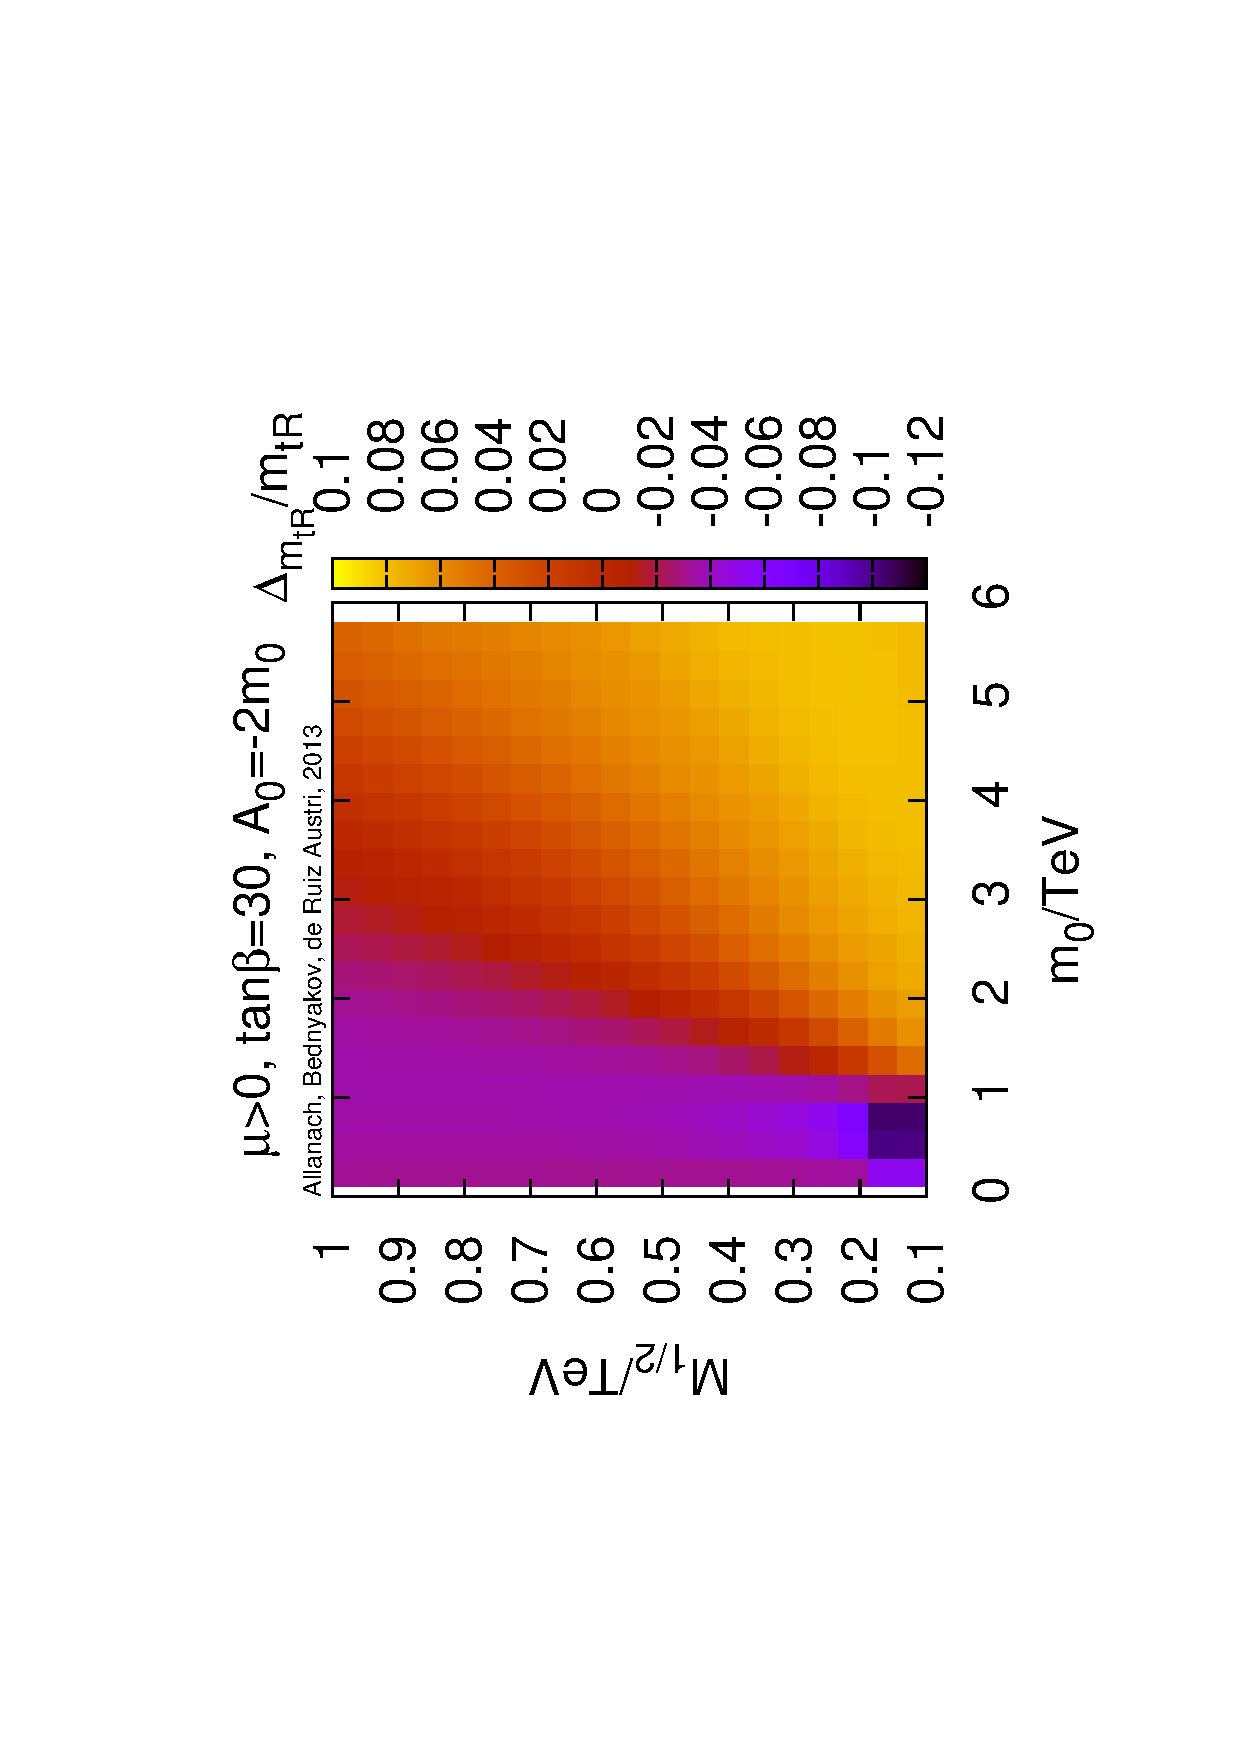
\includegraphics[angle=270,width=0.7\textwidth]{atlasScanMtR}}
  \put(3.22,4.94){
\includegraphics[angle=270,width=0.45\textwidth]{atlasScanMtR2}} 
  \put(3.22,4.94){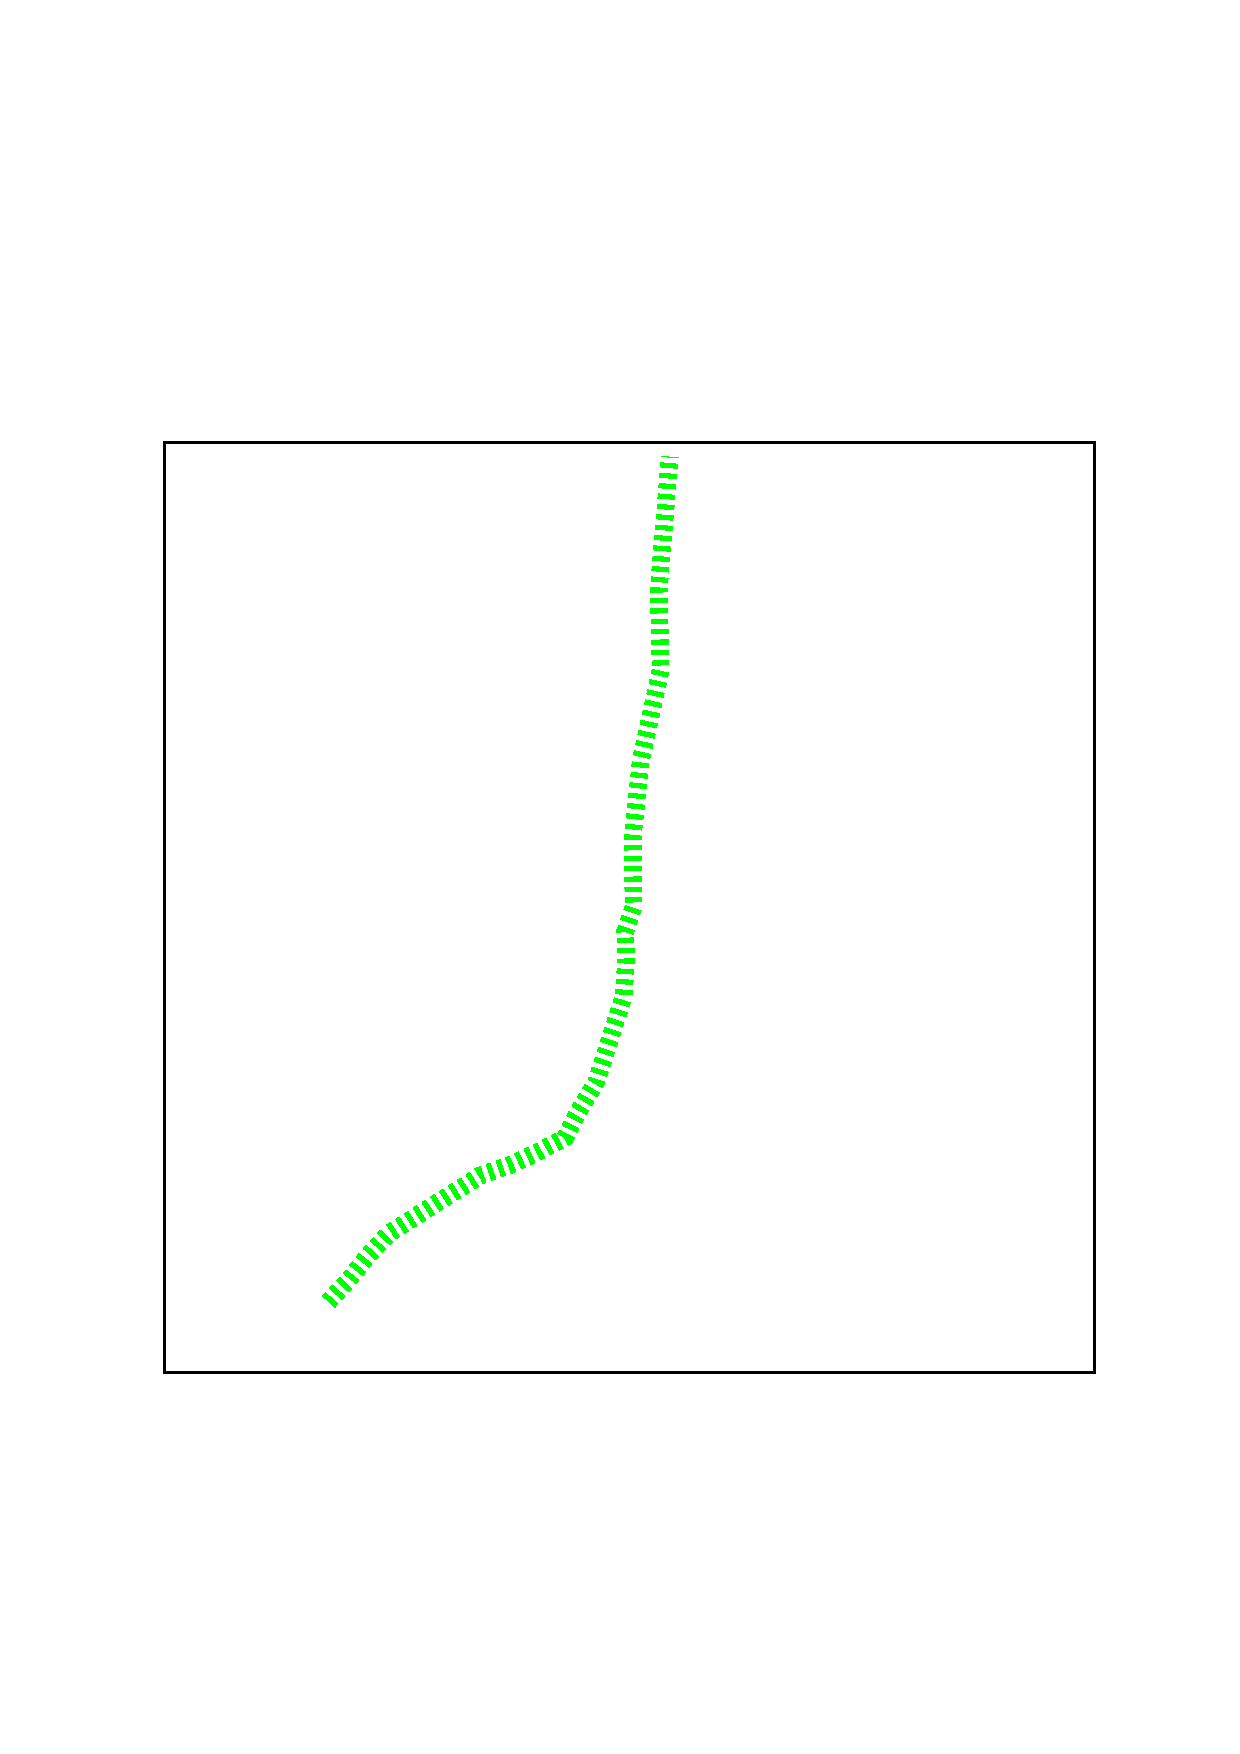
\includegraphics[angle=270,width=0.45\textwidth]{atlasExcl}}
  \put(-0.75,8.2){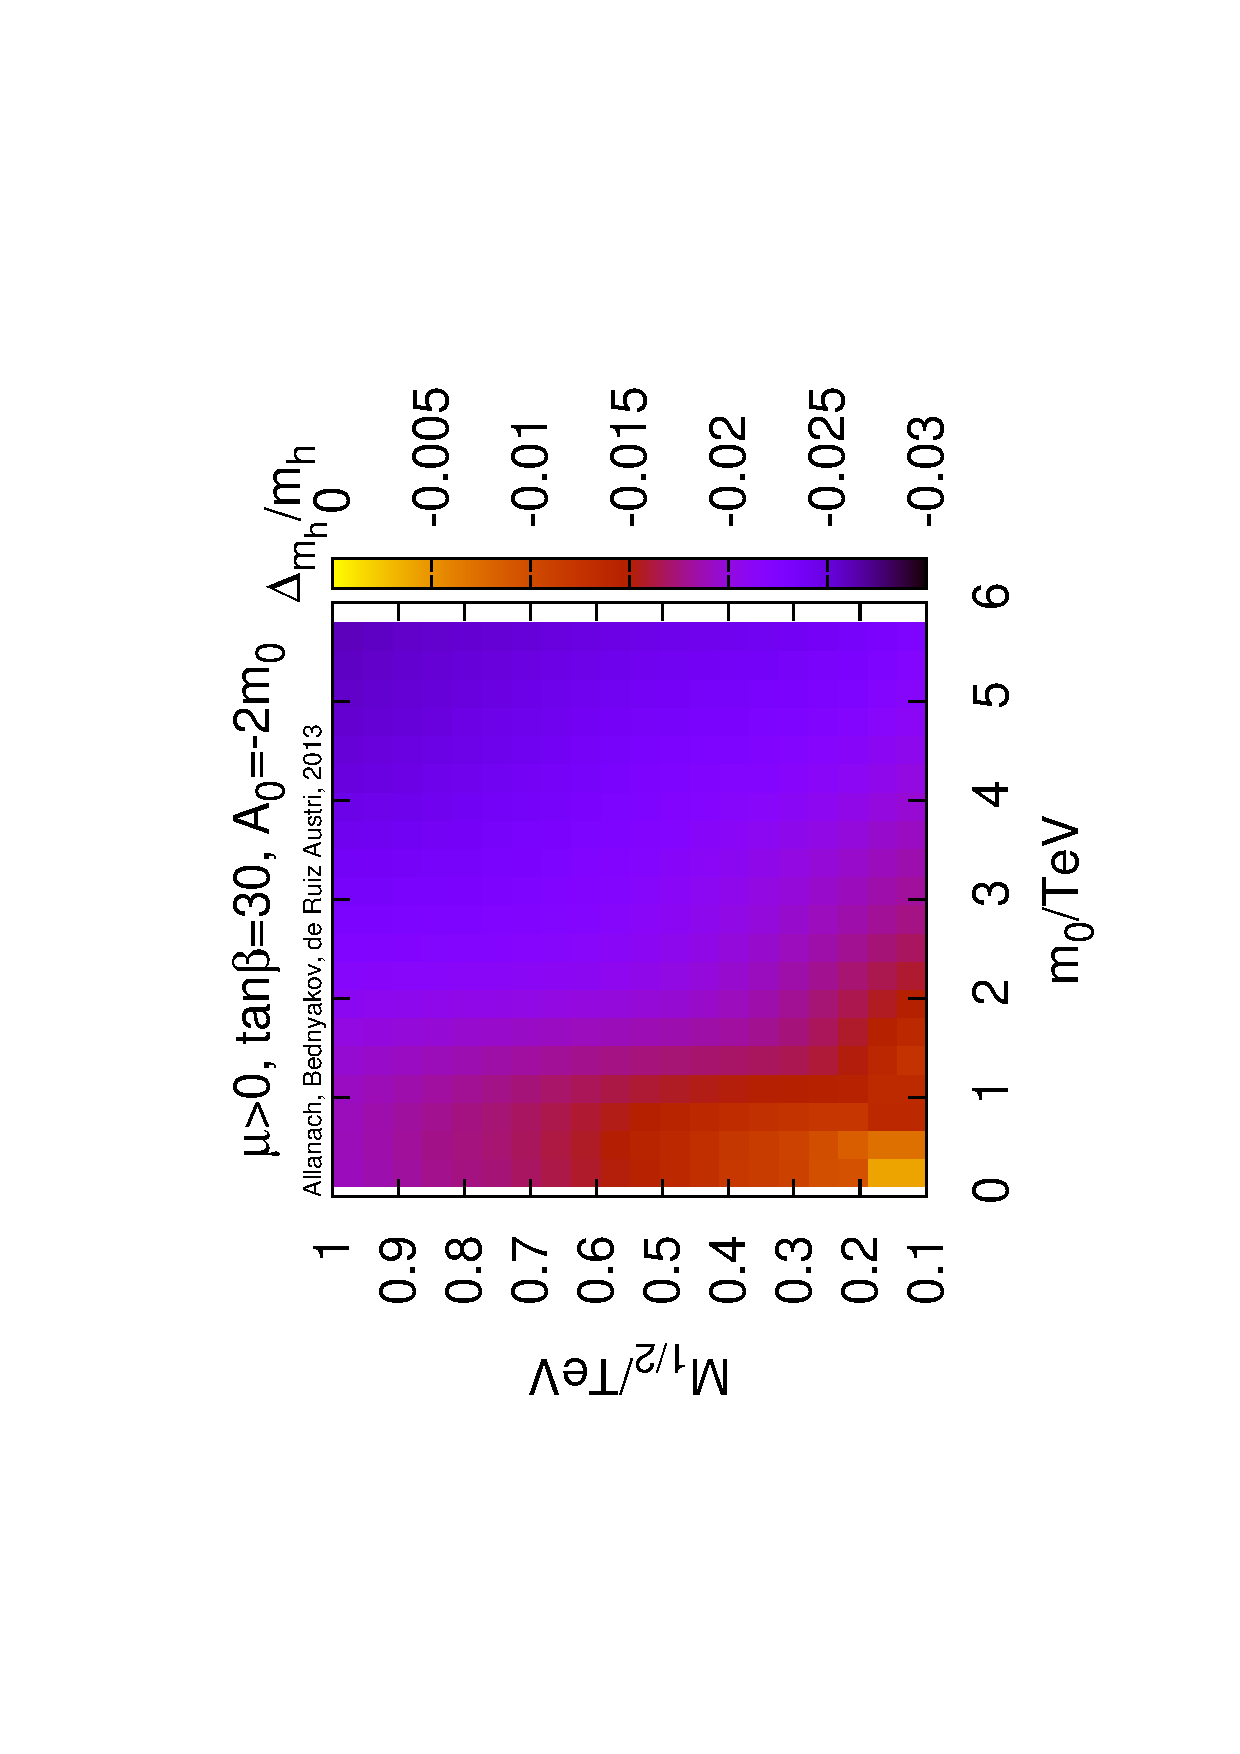
\includegraphics[angle=270,width=0.7\textwidth]{atlasScanMh}}
  \put(0.08,7.64){
\includegraphics[angle=270,width=0.45\textwidth]{atlasScanMh2}}
  \put(0.08,7.64){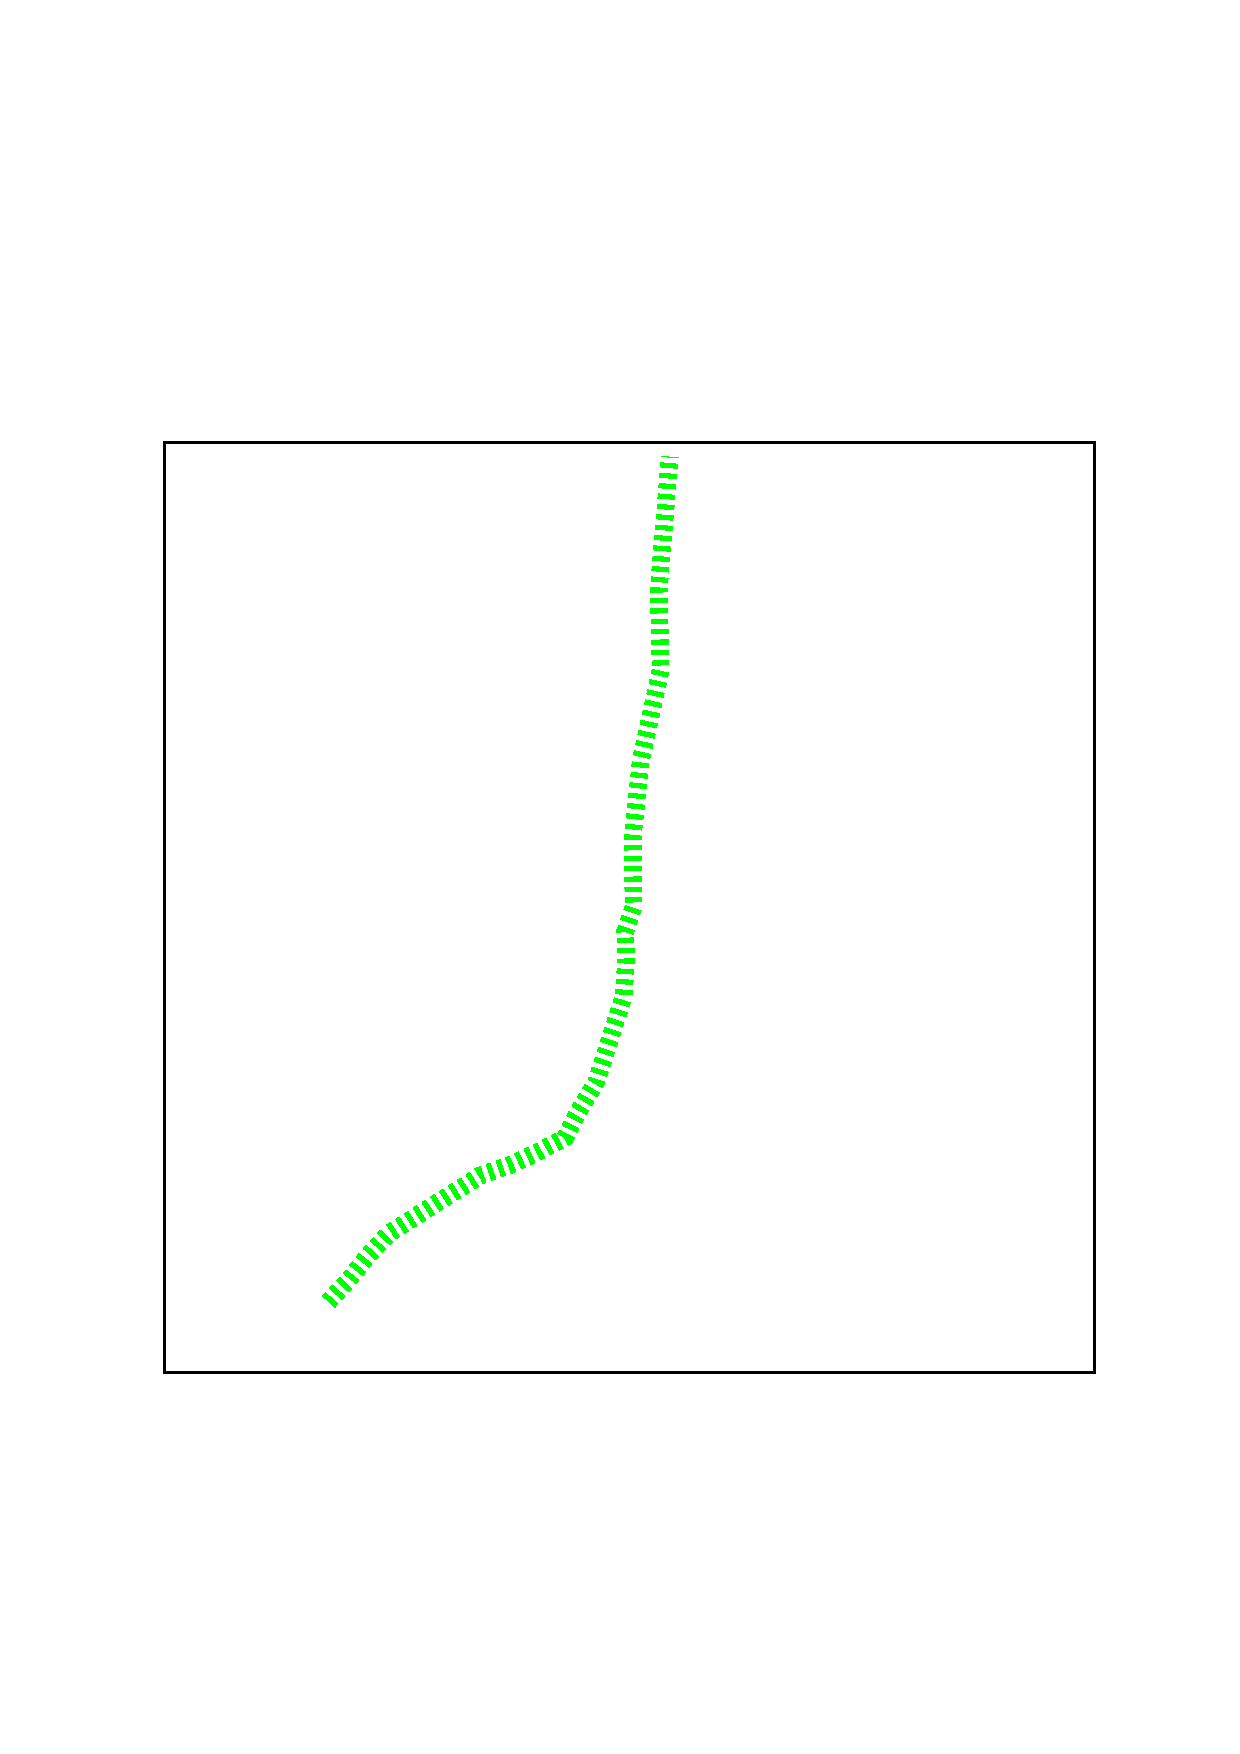
\includegraphics[angle=270,width=0.45\textwidth]{atlasExcl}}
  \put(2.4,8.2){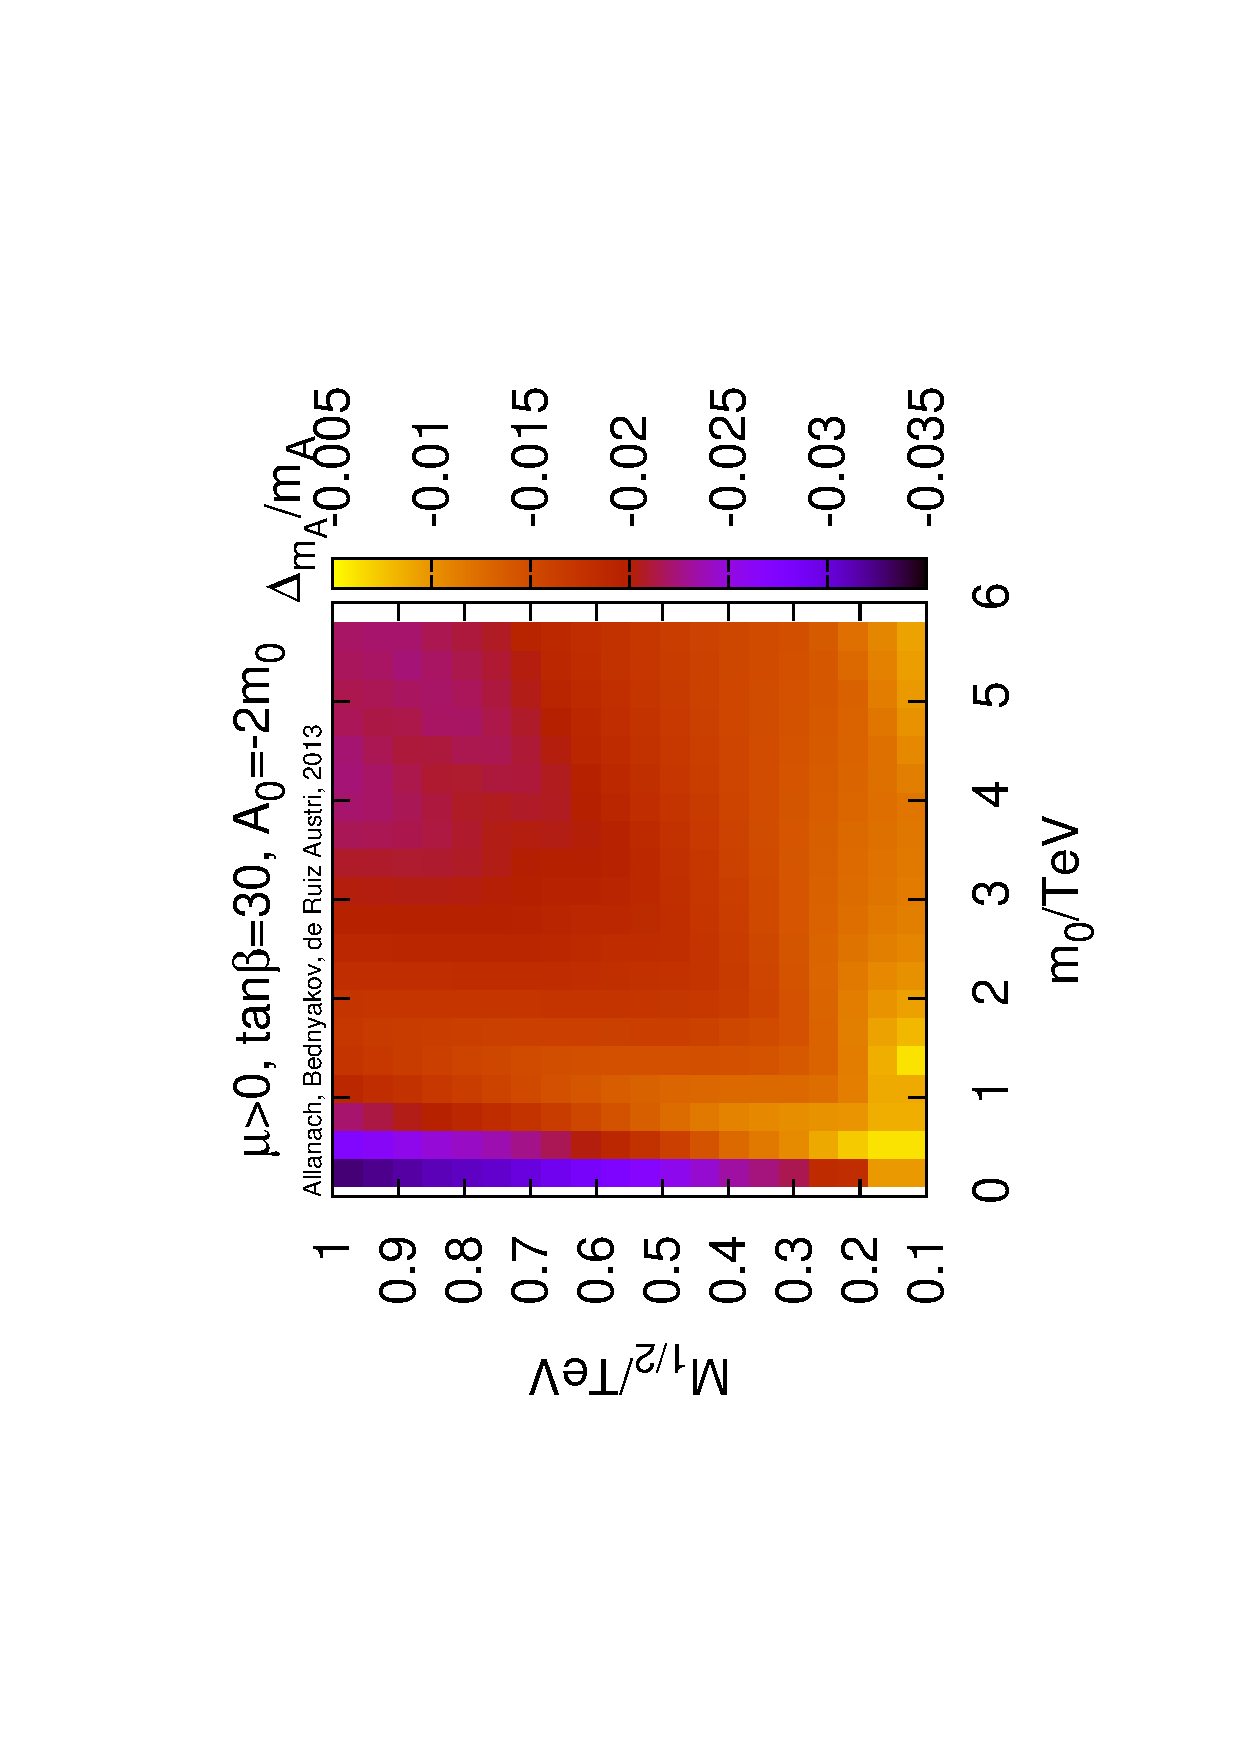
\includegraphics[angle=270,width=0.7\textwidth]{atlasScanMA}}
  \put(3.22,7.64){
\includegraphics[angle=270,width=0.45\textwidth]{atlasScanMA2}}
  \put(3.22,7.64){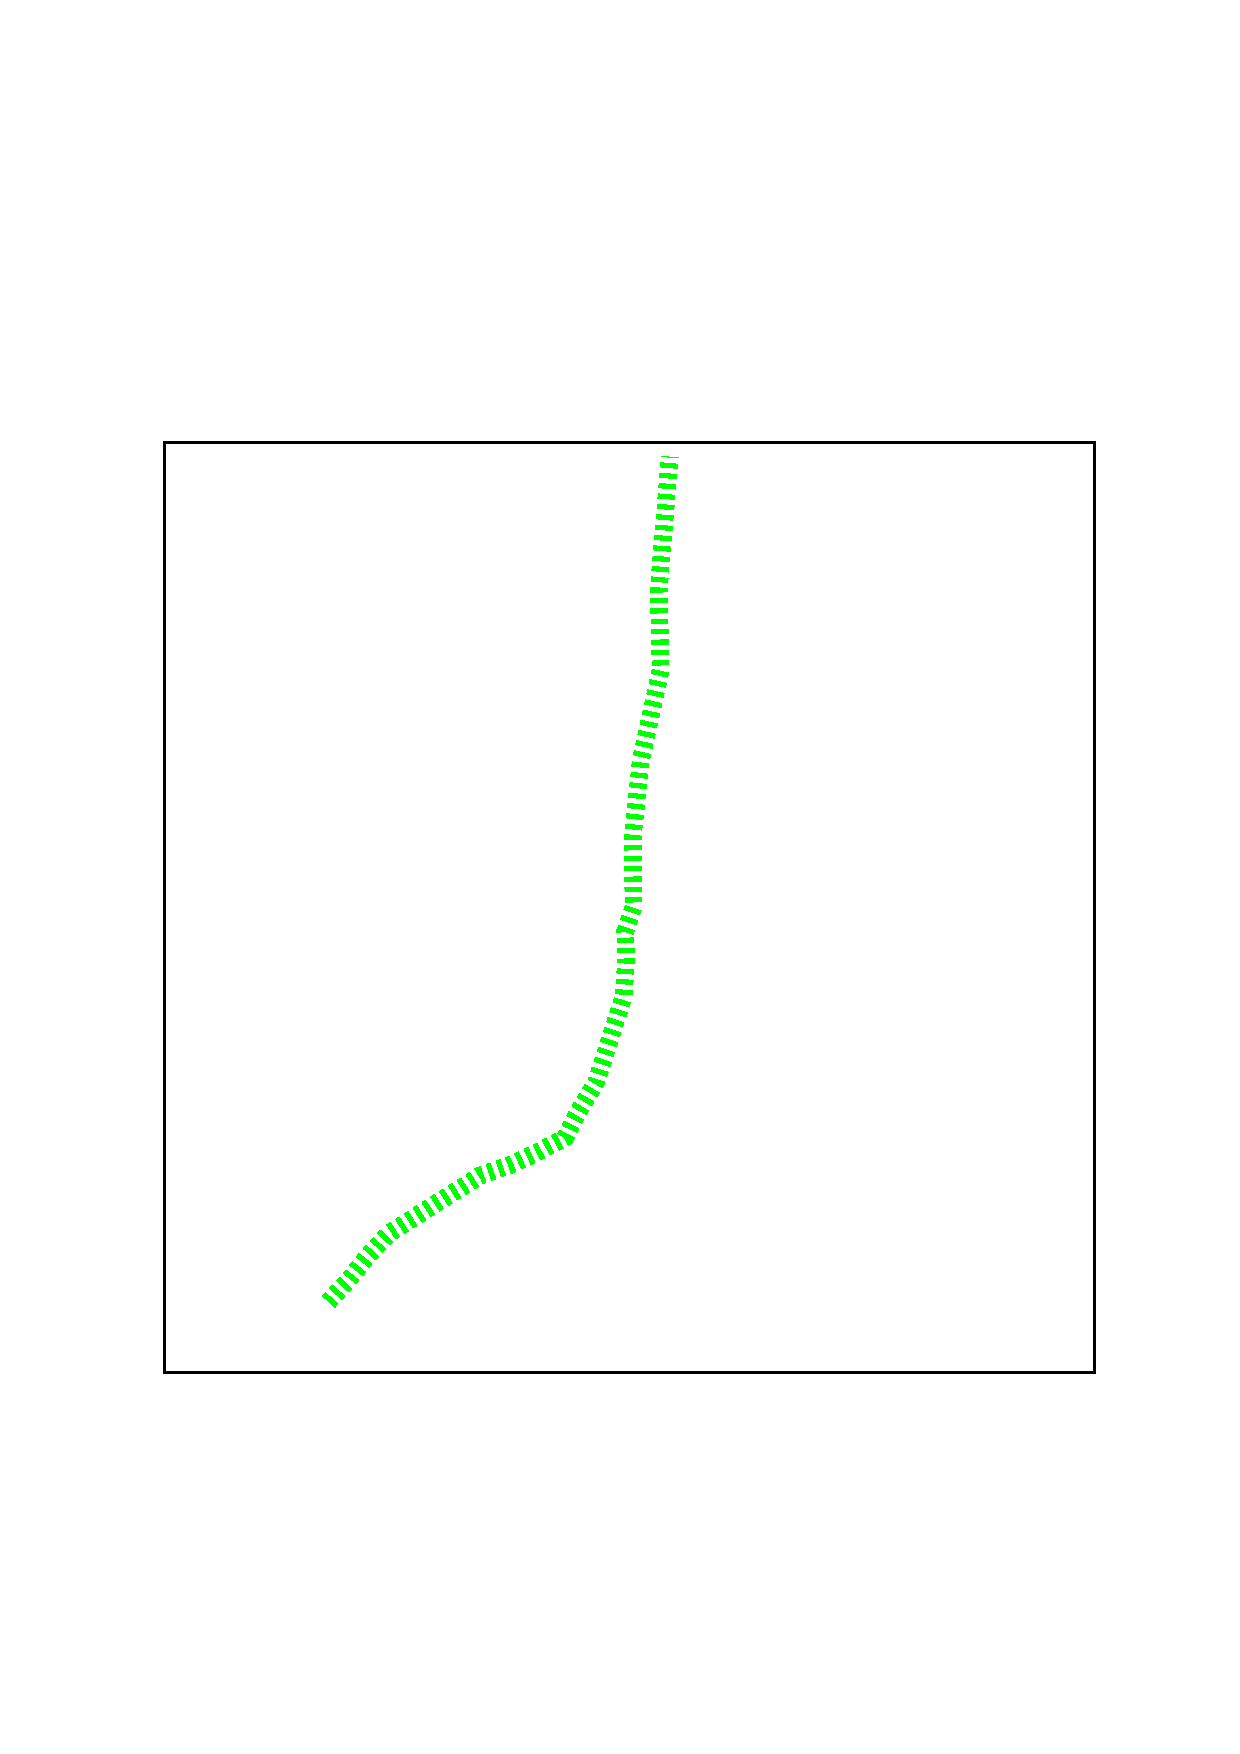
\includegraphics[angle=270,width=0.45\textwidth]{atlasExcl}}
\put(0,7.8){(a)}
\put(3.2,7.8){(b)}
\put(0,5){(c)}
\put(3.2,5){(d)}
\put(0,2.2){(e)}
\put(3.2,2.2){(f)}
\end{picture}
\end{center}
\caption{\label{fig:dm} Relative effect of highest order terms (three-loop
  RGEs for gauge and Yukawa couplings and two-loop threshold corrections to
  third family fermion masses and $g_3$) on various
  particle pole masses in the CMSSM. The CMSSM 
  parameters coincide with the latest ATLAS searches for jets and missing
  energy interpreted in the 
  CMSSM~\cite{ATLAS-CONF-2013-047,Aad:2013wta}.
  Contours of iso-mass are overlayed on each
  figure, with each contour labelling the mass in GeV. Here, $m_g$ denotes the
  gluino mass and $m_q$ the average squark mass from the first two 
  generations.}
\end{figure}

\begin{figure}
\unitlength=1in
\begin{center}
\begin{picture}(3,3)
  \put(-0.75,2.8){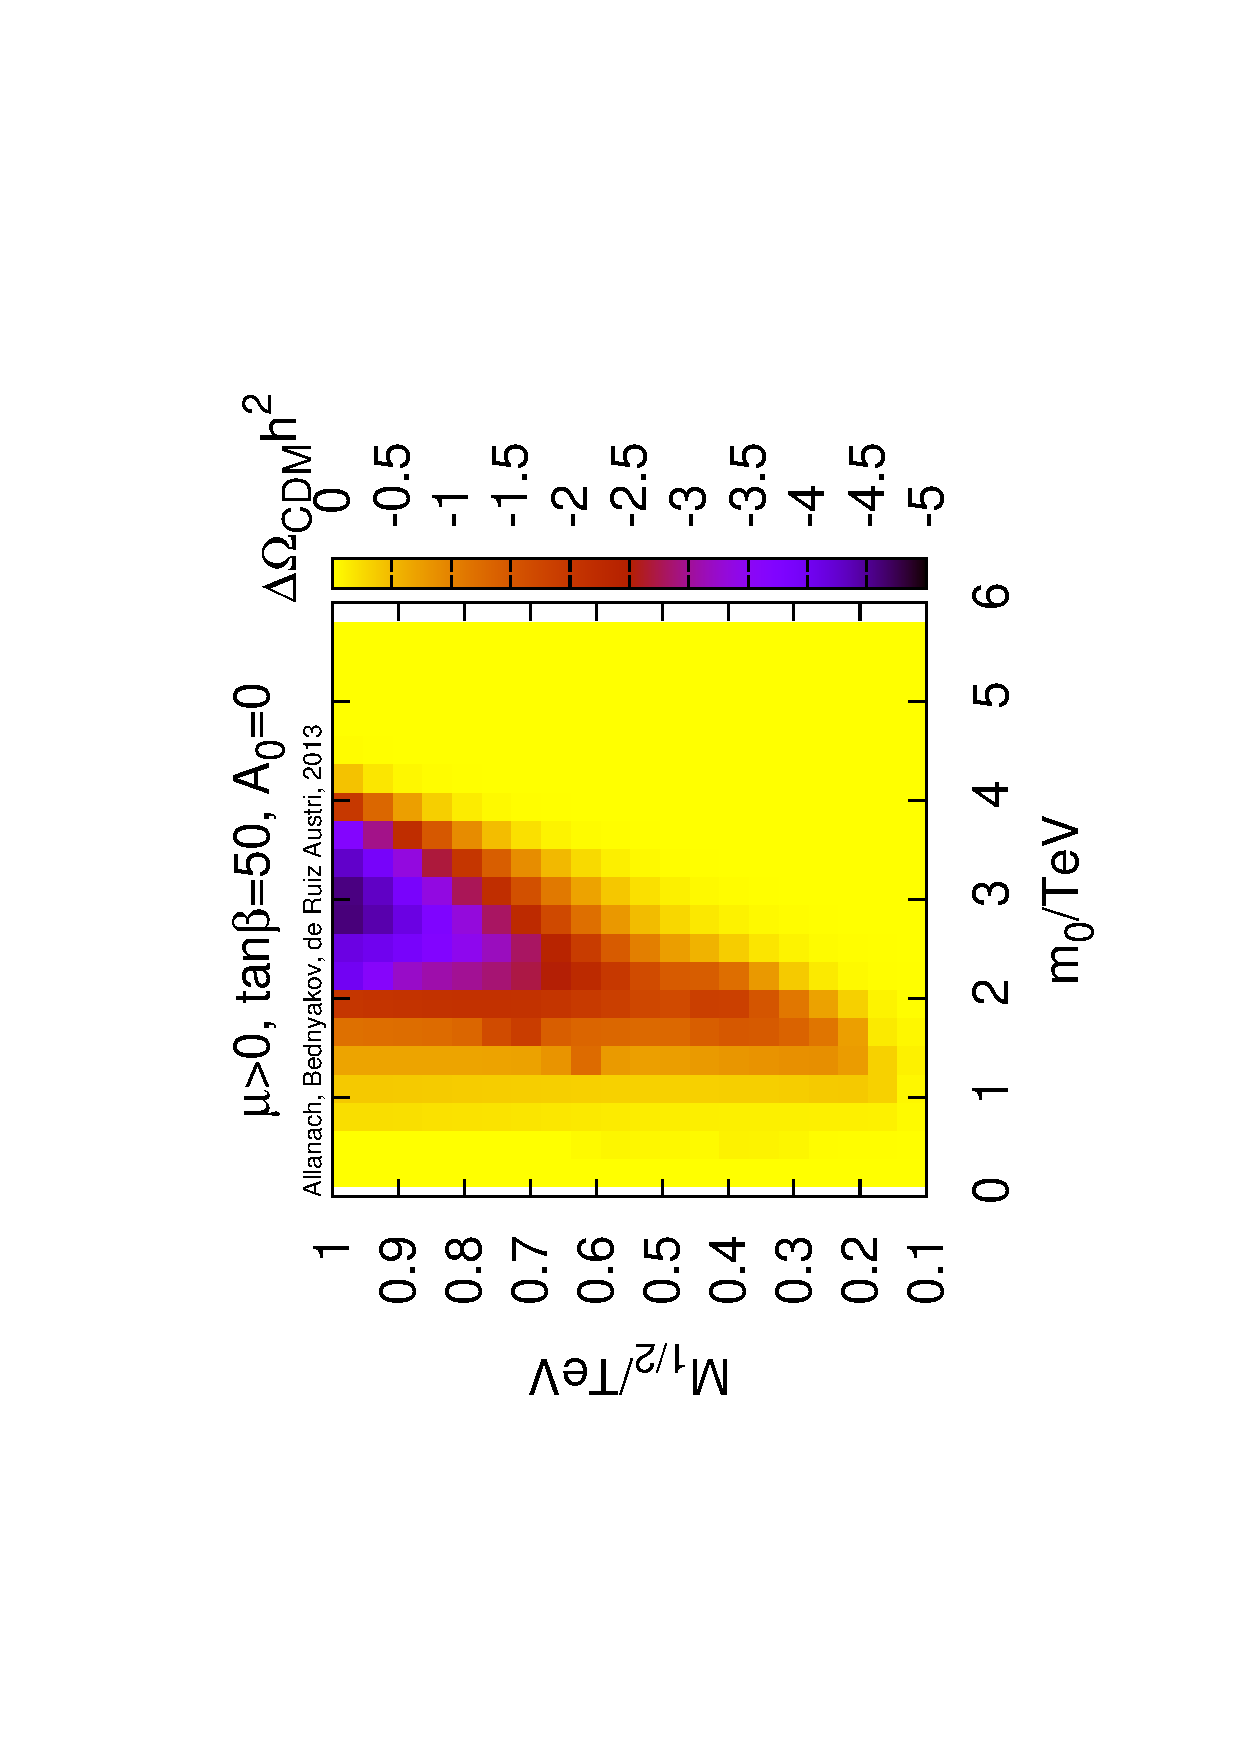
\includegraphics[angle=270,width=0.7\textwidth]{hiTbScanOm}}
  \put(0.08,2.24){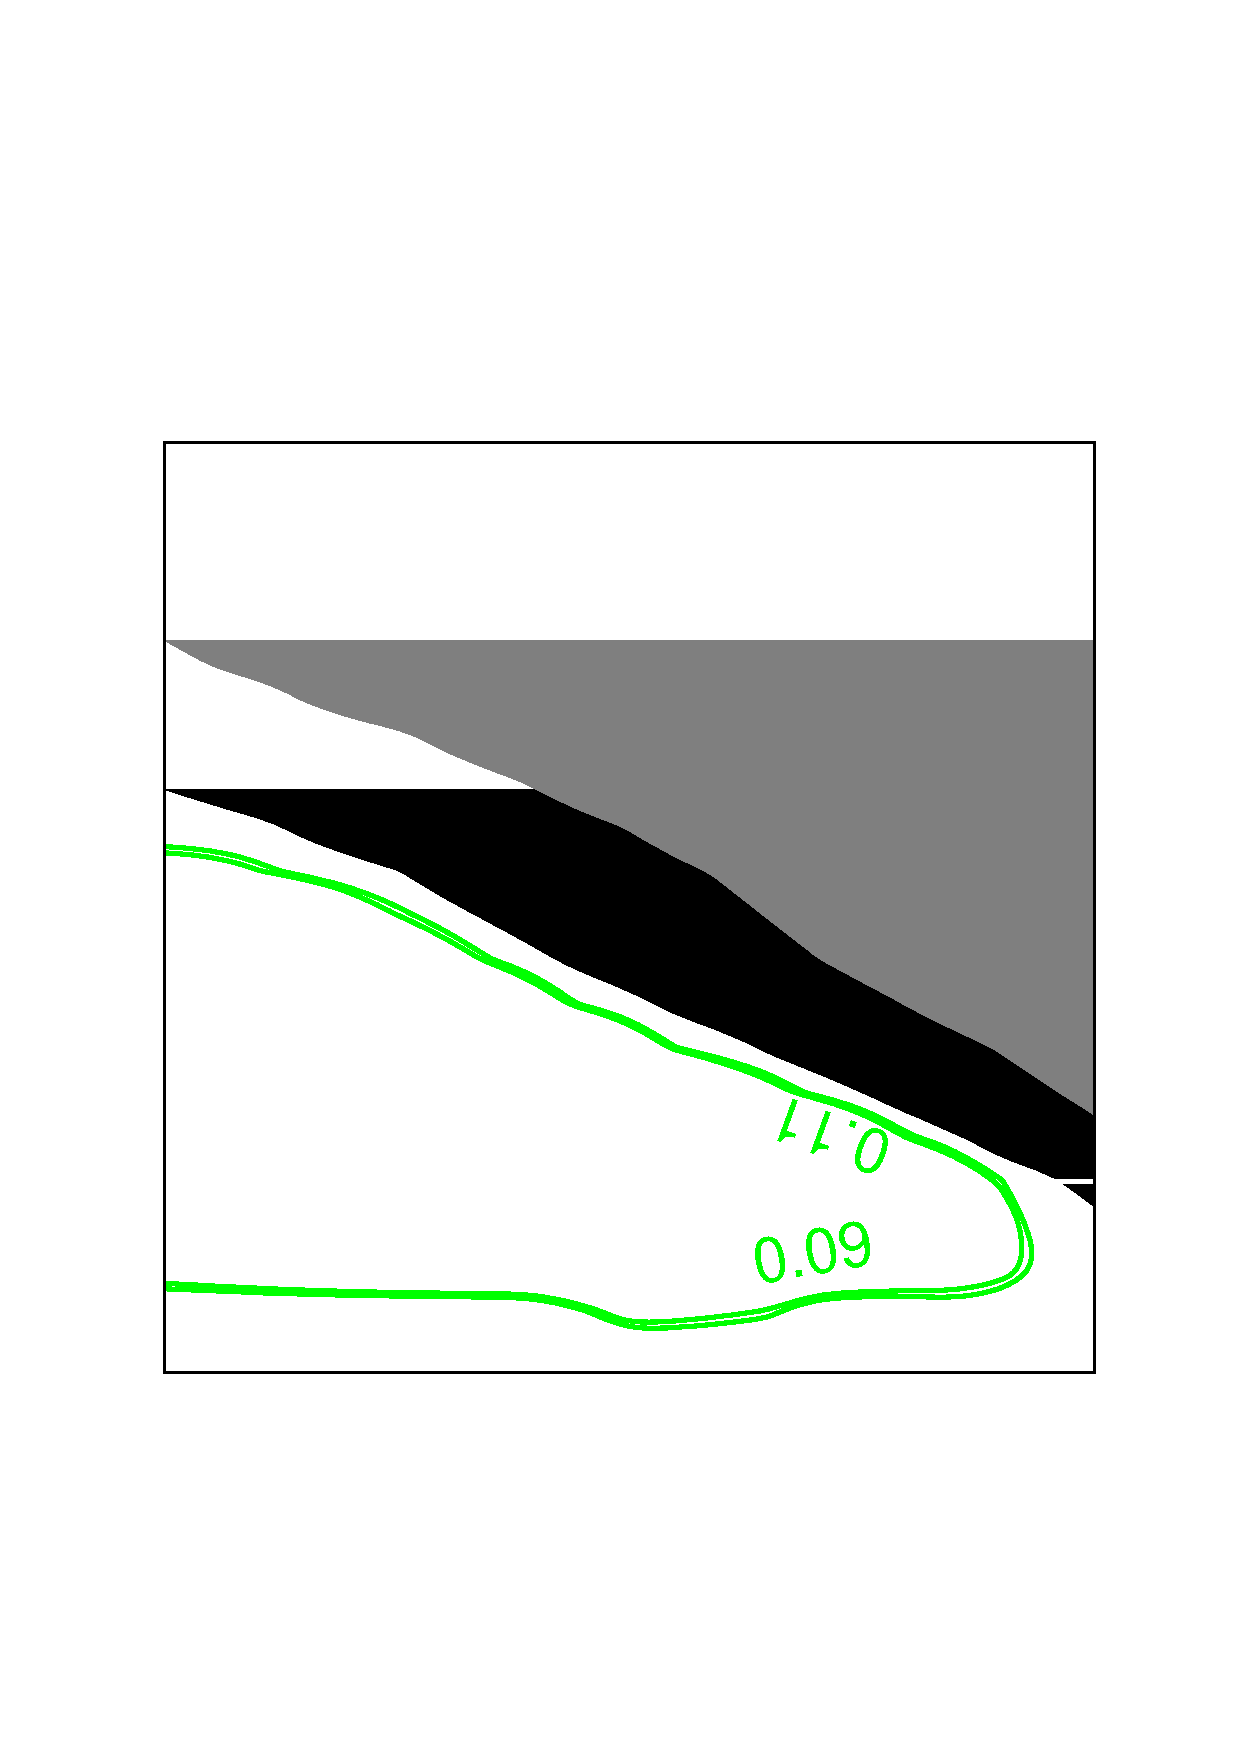
\includegraphics[angle=270,width=0.45\textwidth]{hiTbScanOm2}}
\end{picture}
\end{center}
\caption{\label{fig:dm} Effect of highest order terms (three-loop
  RGEs for gauge and Yukawa couplings and two-loop threshold corrections to
  third family fermion masses and $g_3$) on the predicted dark matter relic
  density in the CMSSM in a high $\tan \beta$ scenario. Contours of iso-relic
  density for the highest order prediction are overlayed. Also shown is the
  change in the position of the border of successful EWSB: the black region
  (and to the right) denotes the region for higher loop corrections, whereas
  the lighter one denotes the result of the standard \SOFTSUSY~calculation.}
\end{figure}




\section{Effect on Unification}


\section*{Acknowledgments}
This work has been partially supported by STFC.

\appendix

\section{Installation of the Increased Accuracy Mode}
\label{sec:install}

Two compilation options are added
\begin{itemize}
	\item[] \verb|--enable-three-loop-rge-compilation| - compile three-loop RGEs in the MSSM 
	\item[] \verb|--enable-full-susy-threshold-compilation| - compile
          additional two-loop threshold corrections to the third generation
          Yukawa couplings and the strong coupling constant.
\end{itemize}

Boolean variables that control the Increased Accuracy Mode at runtime
\begin{itemize}
	\item \verb|USE_THREE_LOOP_RGE = false|  - add three-loop contribution to MSSM RGE (corresponds to the \code{SOFTSUSY Block} parameter 19)
	\item \verb|USE_TWO_LOOP_THRESHOLD = false| - add two-loop threshold corrections to the third generation Yukawa couplings and the strong coupling constant
(corresponds to the \code{SOFTSUSY Block} parameter 20)
\end{itemize}

Additional variables that gives a finer control the Increased Accuracy Mode at runtime (with their default values)
\begin{itemize}
	\item \verb|double TWOLOOP_NUM_THRESH = 0.1|  - used in the iterative algorithm to prevent lengthy re-evaluation of two-loop thresholds 
		if the relative difference between the result obtained in current step and the  calcululated previously is less than \verb|TWOLOOP_NUM_THRESH| 
	\item \verb|boolean SOFTSUSY_TWOLOOP_blah = true| - control whether individual two-loop threshold corrections should be added (remove it or make a \verb|enum|?)
	\item \verb|boolean MB_DECOUPLING = false| - evaluate b-quark self-energies at $p=0$ in order to incorporate ``decoupling'' precedure (remove it?)
\end{itemize}


\section{Running \SOFTSUSY in the Increased Accuracy Mode} 
\label{sec:run}

\SOFTSUSY~produces an executable called \code{softpoint.x}. For the calculation
of the spectrum of single points in parameter space, we recommend the
SUSY Les Houches Accord 2 (SLHA2)~\cite{Allanach:2008qq}  input/output
option. The user must provide a file (e.g.\ the example file included
in the \SOFTSUSY~distribution
\code{rpvHouchesInput}), that specifies the model dependent input
parameters. The program may then be run with
\small
\begin{verbatim}
 ./softpoint.x leshouches < inOutFiles/lesHouchesInput
\end{verbatim}
\normalsize

One can change whether the 3-loop RGE corrections are switched on with
\code{SOFTSUSY Block} parameter 19, whereas the 2-loop third family and $g_3$
threshold corrections 
are switched on with \code{SOFTSUSY Block} parameter 20 in the SLHA2 input file:
\small
\begin{verbatim}
Block SOFTSUSY               # Optional SOFTSUSY-specific parameters
   19   1.000000000e+00      # Include 3-loop RGE terms (0 to disable)
   20   1.000000000e+00      # Include 2-loop thresholds (0 to disable)
\end{verbatim}
\normalsize


% \begin{thebibliography}{10}
% \bibitem{Aad:2013wta}
%   G.~Aad {\it et al.}  [ATLAS Collaboration],
%   %``Search for new phenomena in final states with large jet multiplicities and missing transverse momentum at $\sqrt{s}=8$ TeV proton-proton collisions using the ATLAS experiment,''
%   JHEP {\bf 1310} (2013) 130
%   [arXiv:1308.1841 [hep-ex]].
%   %%CITATION = ARXIV:1308.1841;%%
%   %10 citations counted in INSPIRE as of 06 Nov 2013
% %\cite{Aad:2012tfa}
% \bibitem{CMSspart}
% S.~Chatrchyan {\it et al.} [CMS Collaboration], (2013) CMS-PAS-SUS-13-012
%     %\cite{Allanach:2008zn}
% \bibitem{Allanach:2008zn}
%   B.~C.~Allanach,
%   %``SUSY Predictions and SUSY Tools at the LHC,''
%   Eur.\ Phys.\ J.\ C {\bf 59} (2009) 427
%   [arXiv:0805.2088 [hep-ph]].
%   %%CITATION = ARXIV:0805.2088;%%
%   %13 citations counted in INSPIRE as of 06 Nov 2013

%   \bibitem{Baer:1993ae}
% H.~Baer, F.~E. Paige, S.~D. Protopopescu and X.~Tata, 
% %{\it {Simulating
% %  Supersymmetry with ISAJET 7.0 / ISASUSY 1.0}},
% [hep-ph/9305342].
% %%CITATION = HEP-PH/9305342;%%
% %\cite{Allanach:2001kg}
% \bibitem{Allanach:2001kg} 
%   B.~C.~Allanach,
%   %``SOFTSUSY: a program for calculating supersymmetric spectra,''
%   Comput.\ Phys.\ Commun.\  {\bf 143}, 305 (2002)
%   [hep-ph/0104145].
%   %%CITATION = HEP-PH/0104145;%%
%   %716 citations counted in INSPIRE as of 20 Sep 2013

% \bibitem{Porod:2003um}
% W.~Porod, 
% %{\it {SPheno, a program for calculating supersymmetric spectra, SUSY
% %  particle decays and SUSY particle production at e+ e- colliders}},  
%   Comput.\ Phys.\ Commun. {\bf 153} (2003) 275--315
%   [hep-ph/0301101].
% %%CITATION = HEP-PH/0301101;%%
% \bibitem{Chowdhury:2011zr}
% D.~Chowdhury, R.~Garani and S.~K. Vempati, 
% %{\it {SUSEFLAV: Program for
% %  supersymmetric mass spectra with seesaw mechanism and rare lepton flavor
% %  violating decays}},  
% Comput.\ Phys.\ Commun. {\bf 184} (2013) 899--918
%   [arXiv:1109.3551 [hep-ph]].
% %%CITATION = ARXIV:1109.3551;%%

% \bibitem{Djouadi:2002ze}
% A.~Djouadi, J.-L. Kneur and G.~Moultaka, 
% %{\it {SuSpect: A Fortran code for the
% %  supersymmetric and Higgs particle spectrum in the MSSM}},  
%   Comput.\ Phys.\ Commun. {\bf 176} (2007) 426--455
%   [hep-ph/0211331].
% %%CITATION = HEP-PH/0211331;%%
% %\cite{Djouadi:2013lra}

% %\cite{Skands:2003cj}
% \bibitem{Skands:2003cj}
%   P.~Z.~Skands, B.~C.~Allanach, H.~Baer, C.~Balazs, G.~Belanger, F.~Boudjema, A.~Djouadi and R.~Godbole {\it et al.},
%   %``SUSY Les Houches accord: Interfacing SUSY spectrum calculators, decay packages, and event generators,''
%   JHEP {\bf 0407} (2004) 036
%   [hep-ph/0311123].
%   %%CITATION = HEP-PH/0311123;%%
%   %380 citations counted in INSPIRE as of 07 Nov 2013
% \bibitem{Aad:2012tfa}
%   G.~Aad {\it et al.}  [ATLAS Collaboration],
%   %``Observation of a new particle in the search for the Standard Model Higgs boson with the ATLAS detector at the LHC,''
%   Phys.\ Lett.\ B {\bf 716} (2012) 1
%   [arXiv:1207.7214 [hep-ex]].
%   %%CITATION = ARXIV:1207.7214;%%
%   %1868 citations counted in INSPIRE as of 06 Nov 2013
% %\cite{Chatrchyan:2012ufa}
% \bibitem{Chatrchyan:2012ufa}
%   S.~Chatrchyan {\it et al.}  [CMS Collaboration],
%   %``Observation of a new boson at a mass of 125 GeV with the CMS experiment at the LHC,''
%   Phys.\ Lett.\ B {\bf 716} (2012) 30
%   [arXiv:1207.7235 [hep-ex]].
%   %%CITATION = ARXIV:1207.7235;%%
%   %1848 citations counted in INSPIRE as of 06 Nov 2013

% \bibitem{ATLAS-CONF-2013-014}
% G.~Aad {\it et al.}  [ATLAS Collaboration],
% ATLAS-CONF-2013-014, talk delivered at 48th Rencontres de Moriond on Electroweak Interactions and Unified Theories, La Thuile, Italy, 2 - 9 Mar 2013.


% \bibitem{Djouadi:2013lra}
%   A.~Djouadi,
%   %``Implications of the Higgs discovery for the MSSM,''
%   arXiv:1311.0720 [hep-ph].
%   %%CITATION = ARXIV:1311.0720;%%

% \bibitem{Barbieri:1998uv}
%   R.~Barbieri and A.~Strumia,
%   %``About the fine tuning price of LEP,''
%   Phys.\ Lett.\ B {\bf 433} (1998) 63
%   [hep-ph/9801353].
%   %%CITATION = HEP-PH/9801353;%%
%   %94 citations counted in INSPIRE as of 07 Nov 2013

% %\cite{Arbey:2011ab}
% \bibitem{Arbey:2011ab}
%   A.~Arbey, M.~Battaglia, A.~Djouadi, F.~Mahmoudi and J.~Quevillon,
%   %``Implications of a 125 GeV Higgs for supersymmetric models,''
%   Phys.\ Lett.\ B {\bf 708} (2012) 162
%   [arXiv:1112.3028 [hep-ph]].
%   %%CITATION = ARXIV:1112.3028;%%
%   %188 citations counted in INSPIRE as of 07 Nov 2013
% %\cite{Delgado:2010uj}
% \bibitem{Delgado:2010uj}
%   A.~Delgado, C.~Kolda, J.~P.~Olson and A.~de la Puente,
%   %``Solving the Little Hierarchy Problem with a Singlet and Explicit $\mu$ Terms,''
%   Phys.\ Rev.\ Lett.\  {\bf 105} (2010) 091802
%   [arXiv:1005.1282 [hep-ph]].
%   %%CITATION = ARXIV:1005.1282;%%
%   %38 citations counted in INSPIRE as of 07 Nov 2013
% \bibitem{Ellwanger:2011mu}
%   U.~Ellwanger, G.~Espitalier-Noel and C.~Hugonie,
%   %``Naturalness and Fine Tuning in the NMSSM: Implications of Early LHC Results,''
%   JHEP {\bf 1109} (2011) 105
%   [arXiv:1107.2472 [hep-ph]].
%   %%CITATION = ARXIV:1107.2472;%%
%   %42 citations counted in INSPIRE as of 07 Nov 2013
% %\cite{King:2012tr}
% \bibitem{King:2012tr}
%   S.~F.~King, M.~Mühlleitner, R.~Nevzorov and K.~Walz,
%   %``Natural NMSSM Higgs Bosons,''
%   Nucl.\ Phys.\ B {\bf 870} (2013) 323
%   [arXiv:1211.5074 [hep-ph]].
%   %%CITATION = ARXIV:1211.5074;%%
%   %36 citations counted in INSPIRE as of 07 Nov 2013
% %\cite{Perelstein:2012qg}
% \bibitem{Perelstein:2012qg}
%   M.~Perelstein and B.~Shakya,
%   %``XENON100 Implications for Naturalness in the MSSM, NMSSM and lambda-SUSY,''
%   Phys.\ Rev.\ D {\bf 88} (2013) 075003
%   [arXiv:1208.0833 [hep-ph]].
%   %%CITATION = ARXIV:1208.0833;%%
%   %29 citations counted in INSPIRE as of 07 Nov 2013
% %\cite{Ross:2011xv}
% %\cite{Gherghetta:2012gb}
% \bibitem{Gherghetta:2012gb} 
%   T.~Gherghetta, B.~von Harling, A.~D.~Medina and M.~A.~Schmidt,
%   %``The Scale-Invariant NMSSM and the 126 GeV Higgs Boson,''
%   JHEP {\bf 02}, 032 (2013)
%   [arXiv:1212.5243 [hep-ph]].
%   %%CITATION = ARXIV:1212.5243;%%
%   %33 citations counted in INSPIRE as of 29 Nov 2013
% %\cite{BasteroGil:2000bw}
% \bibitem{BasteroGil:2000bw}
%   M.~Bastero-Gil, C.~Hugonie, S.~F.~King, D.~P.~Roy and S.~Vempati,
%   %``Does LEP prefer the NMSSM?,''
%   Phys.\ Lett.\ B {\bf 489} (2000) 359
%   [hep-ph/0006198].
%   %%CITATION = HEP-PH/0006198;%%
%   %141 citations counted in INSPIRE as of 07 Nov 2013

% %\cite{Ellwanger:2009dp}
% \bibitem{Ellwanger:2009dp}
%   U.~Ellwanger, C.~Hugonie and A.~M.~Teixeira,
%   %``The Next-to-Minimal Supersymmetric Standard Model,''
%   Phys.\ Rept.\  {\bf 496} (2010) 1
%   [arXiv:0910.1785 [hep-ph]].
%   %%CITATION = ARXIV:0910.1785;%%
%   %344 citations counted in INSPIRE as of 07 Nov 2013

% %\cite{Maniatis:2009re}
% \bibitem{Maniatis:2009re} 
%   M.~Maniatis,
%   %``The Next-to-Minimal Supersymmetric extension of the Standard Model reviewed,''
%   Int.\ J.\ Mod.\ Phys.\ A {\bf 25}, 3505 (2010)
%   [arXiv:0906.0777 [hep-ph]].
%   %%CITATION = ARXIV:0906.0777;%%
%   %137 citations counted in INSPIRE as of 29 Nov 2013


% \bibitem{NMSSM} P. Fayet, Nucl. Phys. B \textbf{90} (1975) 104; Phys. Lett.
% B \textbf{64} (1976) 159; Phys. Lett. B \textbf{69} (1977) 489 and Phys. Lett. B
% \textbf{84} (1979) 416; H.P. Nilles, M. Srednicki and D. Wyler, Phys. Lett. B
% \textbf{120} (1983) 346; J.M. Frere, D.R. Jones and S. Raby, Nucl. Phys. B
% \textbf{222} (1983) 11; J.P. Derendinger and C.A. Savoy, Nucl. Phys. B
% \textbf{237} (1984) 307;  A.I. Veselov, M.I. Vysotsky and K.A. Ter-Martirosian,
% Sov. Phys. JETP \textbf{63} (1986) 489; J.R. Ellis, J.F. Gunion, H.E. Haber, L.
% Roszkowski and F. Zwirner, Phys. Rev. D \textbf{39}  (1989) 844; M. Drees, Int.
% J. Mod. Phys. A \textbf{4}  (1989) 3635; U. Ellwanger, M. Rausch de
% Traubenberg and C.A. Savoy, Phys. 
% Lett. B \textbf{315} (1993) 331, Z. Phys. C {\bf 67} (1995) 665 and Nucl. Phys.
% B \textbf{492} (1997) 307; U.~Ellwanger, Phys.\ Lett.\  B {\bf 303} (1993) 271; P.
% Pandita, Z. Phys. C \textbf{59} (1993) 575; T. Elliott, S.F. King and P.L.
% White, Phys. Rev. D {\bf 49} (1994) 2435; S.F. King and P.L. White, Phys. Rev. D
% \textbf{52} (1995) 4183;  F.~Franke and H.~Fraas, Int.\ J.\ Mod.\ Phys.\  A {\bf
% 12} (1997) 479.   D.~J.~Miller, R.~Nevzorov and P.~M.~Zerwas,  Nucl.\ Phys.\ B {\bf 681}, 3 (2004) [hep-ph/0304049].

% %\cite{Ell08}
% \bibitem{Ell08} 
%   U.~Ellwanger, C.~-C.~Jean-Louis and A.~M.~Teixeira,
%   %``Phenomenology of the General NMSSM with Gauge Mediated Supersymmetry Breaking,''
%   JHEP {\bf 0805}, 044 (2008)
%   [arXiv:0803.2962 [hep-ph]].
%   %%CITATION = ARXIV:0803.2962;%%
%   %28 citations counted in INSPIRE as of 24 Sep 2013


% \bibitem{Ross:2011xv}
%   G.~G.~Ross and K.~Schmidt-Hoberg,
%   %``The Fine-Tuning of the Generalised NMSSM,''
%   Nucl.\ Phys.\ B {\bf 862} (2012) 710
%   [arXiv:1108.1284 [hep-ph]].
%   %%CITATION = ARXIV:1108.1284;%%
%   %54 citations counted in INSPIRE as of 07 Nov 2013
% \bibitem{Ross:2012nr}
%   G.~G.~Ross, K.~Schmidt-Hoberg and F.~Staub,
%   %``The Generalised NMSSM at One Loop: Fine Tuning and Phenomenology,''
%   JHEP {\bf 1208} (2012) 074
%   [arXiv:1205.1509 [hep-ph]].
%   %%CITATION = ARXIV:1205.1509;%%
%   %37 citations counted in INSPIRE as of 07 Nov 2013

% %\cite{King:2012is}
% \bibitem{King:2012is}
%   S.~F.~King, M.~Muhlleitner and R.~Nevzorov,
%   %``NMSSM Higgs Benchmarks Near 125 GeV,''
%   Nucl.\ Phys.\ B {\bf 860} (2012) 207
%   [arXiv:1201.2671 [hep-ph]].
%   %%CITATION = ARXIV:1201.2671;%%
%   %106 citations counted in INSPIRE as of 29 Nov 2013

% %\cite{Ellwanger:2006rn}
% \bibitem{Ellwanger:2006rn}
%   U.~Ellwanger and C.~Hugonie,
%   %``NMSPEC: A Fortran code for the sparticle and Higgs masses in the NMSSM with GUT scale boundary conditions,''
%   Comput.\ Phys.\ Commun.\  {\bf 177} (2007) 399
%   [hep-ph/0612134].
%   %%CITATION = HEP-PH/0612134;%%
%   %81 citations counted in INSPIRE as of 07 Nov 2013
% %\cite{Staub:2009bi}
% \bibitem{Staub:2009bi} 
%   F.~Staub,
%   %``From Superpotential to Model Files for FeynArts and CalcHep/CompHep,''
%   Comput.\ Phys.\ Commun.\  {\bf 181}, 1077 (2010)
%   [arXiv:0909.2863 [hep-ph]].
%   %%CITATION = ARXIV:0909.2863;%%
%   %64 citations counted in INSPIRE as of 12 Oct 2013

% %\cite{Staub:2010jh}
% \bibitem{Staub:2010jh} 
%   F.~Staub,
%   %``Automatic Calculation of supersymmetric Renormalization Group Equations and Self Energies,''
%   Comput.\ Phys.\ Commun.\  {\bf 182}, 808 (2011)
%   [arXiv:1002.0840 [hep-ph]].
%   %%CITATION = ARXIV:1002.0840;%%
%   %60 citations counted in INSPIRE as of 12 Oct 2013

% %\cite{Staub:2012pb}
% \bibitem{Staub:2012pb} 
%   F.~Staub,
%   %``SARAH 3.2: Dirac Gauginos, UFO output, and more,''
%   Computer Physics Communications {\bf 184}, pp. 1792 (2013)
%   [Comput.\ Phys.\ Commun.\  {\bf 184}, 1792 (2013)]
%   [arXiv:1207.0906 [hep-ph]].
%   %%CITATION = ARXIV:1207.0906;%%
%   %19 citations counted in INSPIRE as of 12 Oct 2013

% %\cite{Staub:2013tta}
% \bibitem{Staub:2013tta} 
%   F.~Staub,
%   %``SARAH 4: A tool for (not only SUSY) model builders,''
%   arXiv:1309.7223 [hep-ph].
%   %%CITATION = ARXIV:1309.7223;%%
%   %2 citations counted in INSPIRE as of 12 Oct 2013

% %\cite{Bharucha:2013ela}
% \bibitem{Bharucha:2013ela}
%   A.~Bharucha, A.~Goudelis and M.~McGarrie,
%   %``En-gauging Naturalness,''
%   arXiv:1310.4500 [hep-ph].
%   %%CITATION = ARXIV:1310.4500;%%
%   %2 citations counted in INSPIRE as of 04 Dec 2013

% %\cite{Allanach:2008qq}
% \bibitem{Allanach:2008qq} 
%   B.~C.~Allanach, C.~Balazs, G.~Belanger, M.~Bernhardt, F.~Boudjema, D.~Choudhury, K.~Desch and U.~Ellwanger {\it et al.},
%   %``SUSY Les Houches Accord 2,''
%   Comput.\ Phys.\ Commun.\  {\bf 180}, 8 (2009)
%   [arXiv:0801.0045 [hep-ph]].
%   %%CITATION = ARXIV:0801.0045;%%
%   %177 citations counted in INSPIRE as of 21 Sep 2013
% %\cite{Ellwanger:2005dv}
% \bibitem{Ellwanger:2005dv}
%   U.~Ellwanger and C.~Hugonie,
%   %``NMHDECAY 2.0: An Updated program for sparticle masses, Higgs masses, couplings and decay widths in the NMSSM,''
%   Comput.\ Phys.\ Commun.\  {\bf 175} (2006) 290
%   [hep-ph/0508022].
%   %%CITATION = HEP-PH/0508022;%%
%   %193 citations counted in INSPIRE as of 07 Nov 2013
% %\cite{Muhlleitner:2003vg}
% \bibitem{Muhlleitner:2003vg}
%   M.~Muhlleitner, A.~Djouadi and Y.~Mambrini,
%   %``SDECAY: A Fortran code for the decays of the supersymmetric particles in the MSSM,''
%   Comput.\ Phys.\ Commun.\  {\bf 168} (2005) 46
%   [hep-ph/0311167].
%   %%CITATION = HEP-PH/0311167;%%
%   %204 citations counted in INSPIRE as of 07 Nov 2013
% %\cite{Das:2011dg}
% \bibitem{Das:2011dg}
%   D.~Das, U.~Ellwanger and A.~M.~Teixeira,
%   %``NMSDECAY: A Fortran Code for Supersymmetric Particle Decays in the Next-to-Minimal Supersymmetric Standard Model,''
%   Comput.\ Phys.\ Commun.\  {\bf 183} (2012) 774
%   [arXiv:1106.5633 [hep-ph]].
%   %%CITATION = ARXIV:1106.5633;%%
%   %14 citations counted in INSPIRE as of 07 Nov 2013

% %\cite{Sjostrand:2007gs}
% \bibitem{Sjostrand:2007gs}
%   T.~Sjostrand, S.~Mrenna and P.~Z.~Skands,
%   %``A Brief Introduction to PYTHIA 8.1,''
%   Comput.\ Phys.\ Commun.\  {\bf 178} (2008) 852
%   [arXiv:0710.3820 [hep-ph]].
%   %%CITATION = ARXIV:0710.3820;%%
%   %914 citations counted in INSPIRE as of 06 Nov 2013
% %\cite{Belanger:2008sj}
% \bibitem{Belanger:2008sj}
%   G.~Belanger, F.~Boudjema, A.~Pukhov and A.~Semenov,
%   %``Dark matter direct detection rate in a generic model with micrOMEGAs 2.2,''
%   Comput.\ Phys.\ Commun.\  {\bf 180} (2009) 747
%   [arXiv:0803.2360 [hep-ph]].
%   %%CITATION = ARXIV:0803.2360;%%
%   %349 citations counted in INSPIRE as of 07 Nov 2013
% %\cite{Allanach:2009bv}
% \bibitem{Allanach:2009bv}
%   B.~C.~Allanach and M.~A.~Bernhardt,
%   %``Including R-parity violation in the numerical computation of the spectrum of the minimal supersymmetric standard model: SOFTSUSY,''
%   Comput.\ Phys.\ Commun.\  {\bf 181} (2010) 232
%   [arXiv:0903.1805 [hep-ph]].
%   %%CITATION = ARXIV:0903.1805;%%
%   %22 citations counted in INSPIRE as of 07 Nov 2013
% %\cite{Allanach:2011de}
% \bibitem{Allanach:2011de}
%   B.~C.~Allanach, C.~H.~Kom and M.~Hanussek,
%   %``Computation of Neutrino Masses in R-parity Violating Supersymmetry: SOFTSUSY3.2,''
%   Comput.\ Phys.\ Commun.\  {\bf 183} (2012) 785
%   [arXiv:1109.3735 [hep-ph]].
%   %%CITATION = ARXIV:1109.3735;%%
%   %4 citations counted in INSPIRE as of 07 Nov 2013
% \bibitem{Degrassi:2009yq} 
%   G.~Degrassi and P.~Slavich,
%   %``On the radiative corrections to the neutral Higgs boson masses in the NMSSM,''
%   Nucl.\ Phys.\ B {\bf 825}, 119 (2010)
%   [arXiv:0907.4682 [hep-ph]].
%   %%CITATION = ARXIV:0907.4682;%%
%   %35 citations counted in INSPIRE as of 21 Sep 2013
% %\cite{MV94}
% \bibitem{MV94} 
%   S.~P.~Martin and M.~T.~Vaughn,
%   %``Two loop renormalization group equations for soft supersymmetry breaking couplings,''
%   Phys.\ Rev.\ D {\bf 50}, 2282 (1994)
%   [Erratum-ibid.\ D {\bf 78}, 039903 (2008)]
%   [hep-ph/9311340].
%   %%CITATION = HEP-PH/9311340;%%
%   %568 citations counted in INSPIRE as of 24 Sep 2013

% %\cite{Yam94}
% \bibitem{Yam94} 
%   Y.~Yamada,
%   %``Two loop renormalization group equations for soft SUSY breaking scalar interactions: Supergraph method,''
%   Phys.\ Rev.\ D {\bf 50}, 3537 (1994)
%   [hep-ph/9401241].
%   %%CITATION = HEP-PH/9401241;%%
%   %225 citations counted in INSPIRE as of 24 Sep 2013
% \bibitem{Sper13} 
%   M.~Sperling, D.~St\"ockinger and A.~Voigt,
%   %``Renormalization of vacuum expectation values in spontaneously broken gauge theories,''
%   JHEP {\bf 1307}, 132 (2013)
%   [arXiv:1305.1548 [hep-ph]].
%   %%CITATION = ARXIV:1305.1548;%%
%   %4 citations counted in INSPIRE as of 14 Oct 2013

% \bibitem{Sper13-2} 
%   M.~Sperling, D.~St\"ockinger and A.~Voigt,
%   %``Renormalization of vacuum expectation values in spontaneously broken gauge theories: Two-loop results,''
%   arXiv:1310.7629 [hep-ph].
%   %%CITATION = ARXIV:1310.7629;%%
% \bibitem{Pierce:1997zz}
% D.~M. Pierce, J.~A. Bagger, K.~Matchev, and R.~jie Zhang, {\it Precision
%   corrections in the minimal supersymmetric standard model},  {\em Nucl. Phys.}
%   {\bf B491} (1997) 3--67, 
% [{\tt hep-ph/9606211}].
%   %\cite{Staub:2010ty}
% \bibitem{Staub:2010ty} 
%   F.~Staub, W.~Porod and B.~Herrmann,
%   %``The Electroweak sector of the NMSSM at the one-loop level,''
%   JHEP {\bf 1010}, 040 (2010)
%   [arXiv:1007.4049 [hep-ph]].
%   %%CITATION = ARXIV:1007.4049;%%
%   %28 citations counted in INSPIRE as of 12 Oct 2013
% \bibitem{flexi-susy} 
% P.~Athron, Jae-hyeon Park, D.~Stockinger and A.~Voigt, {\it Flexible Supersymmetry}, In development, \\
% https://github.com/Expander/FlexibleSUSY


















% %
% \end{thebibliography}

\bibliography{threeLoop}
\bibliographystyle{elsarticle-num}
\end{document}
